% =============================================================
%  Grid-forming and grid-following AFE blocks of pwr-control/library: description and user guide
%  pwr-control documentation - compile with pdflatex (twice) from inside this folder:
%      pdflatex grid_forming_following_afe.tex && pdflatex grid_forming_following_afe.tex
%  All figures are TikZ / circuitikz drawn in this file: no external data.
%  The same source is kept in pwr-control/library (library/documentation/grid_forming_following_afe/),
%  where ../../AAA_template_latex_settings/ is a copy of the template of this repository; that copy of
%  the PDF is the one opened by the Help button of the masks of the two blocks.
% =============================================================
\documentclass[11pt,a4paper]{scrartcl}
\ifdefined\PWRCONTROLSETTINGSLOADED
\endinput
\fi
\def\PWRCONTROLSETTINGSLOADED{1}
% ===================== PACKAGES =====================
\usepackage[british]{babel}
\usepackage[tmargin=1in, bmargin=1in, lmargin=0.75in, rmargin=0.75in]{geometry}
\usepackage[dvipsnames,table]{xcolor}  % prima di tikz, listings, ecc.

\usepackage{tikz}
\usepackage{graphicx}
\usepackage{pgfplots}
\pgfplotsset{width=12cm, compat=1.9}
\usepackage{setspace}
\usepackage{chemmacros}
\usepackage{chemfig}
\usepackage{tabularray}
\usepackage{makeidx}
\usepackage{epstopdf}
\usepackage{amssymb}
\usepackage{mathrsfs}
\usepackage{bm}
\usepackage{amsmath}
% esint deve essere caricato DOPO amsmath: entrambi definiscono \iint, \iiint,
% \iiiint e \idotsint. Le si rende indefinite in modo che esint le ridefinisca
% (versioni con i simboli di integrale multiplo corretti) senza errori.
\let\iint\undefined
\let\iiint\undefined
\let\iiiint\undefined
\let\idotsint\undefined
\usepackage{esint}
\usepackage{enumitem}
%\usepackage[english]{varioref}
\usepackage{physics}
\usepackage{lipsum}
\usepackage{fancyhdr}
\usepackage{float}
\usepackage{empheq}
\usepackage[framemethod=tikz]{mdframed}
\numberwithin{equation}{section}
\usepackage{eso-pic}
\usepackage{calc}
\usepackage{nccmath}
\usepackage{caption}
\usepackage{subcaption}
\usepackage{gensymb}
\usepackage{amsfonts, amsthm, epsfig, epstopdf, titling, url, array}
\usepackage{tabularx}
\usepackage{makecell}
\usepackage{booktabs}
\usepackage{array}
\usepackage{siunitx}
\sisetup{input-digits=0123456789\pi}
\usepackage[symbol]{footmisc}
\usepackage{multicol}
%\usepackage{boondox-cal}
\usepackage{blindtext}
\usepackage{changepage}
\usepackage{nomencl}
\usepackage{hyperref}
\usepackage{xurl}
\usepackage{ragged2e}
\usepackage[version=4]{mhchem}  % ← conflitto di opzioni
\usepackage{longtable}
\usepackage{chemformula}
\usetikzlibrary{arrows.meta,positioning,calc}
\usepackage[page,toc]{appendix}


% ===================== SI UNITS =====================
\DeclareSIUnit\atm{atm}
\DeclareSIUnit{\var}{var}
\DeclareSIUnit{\pu}{p.u.}
\sisetup{detect-weight=true, detect-inline-weight=math}

% ===================== MATH OPERATORS =====================
%\DeclareMathOperator{\rank}{rank}
\DeclareMathOperator{\atantwo}{atan2}
\DeclareMathOperator{\spn}{span}

% ===================== COMMANDS =====================
%\newcommand{\abs}[1]{\left|#1\right|}
\newcommand{\sign}{\text{sign}}
\newcommand{\centered}[1]{\begin{tabular}{@{}l@{}} #1 \end{tabular}}

% ===================== COLORS =====================
\definecolor{mycolor1}{rgb}{0.97, 0.97, 0.97}
\definecolor{mycolor2}{rgb}{0.97, 0.97, 0.97}
\definecolor{tableShade}{gray}{0.9}

% ===================== THEOREM ENVIRONMENTS =====================
\theoremstyle{it}
\newtheorem{defn}{Definition}[section]
\newtheorem{assumption}{Assumption}[section]
\newtheorem{thm}{Theorem}[section]
\newtheorem{lemma}{Lemma}[section]
\newtheorem{corollary}{Corollary}[section]
\theoremstyle{definition}
\newtheorem{example}{Example}[section]

% ===================== CUSTOM ENVIRONMENTS =====================
\newenvironment{myitemize_1}{
	\begin{itemize}[topsep=0pt]
		\setlength{\topsep}{2pt}
		\setlength{\itemsep}{2pt}
		\setlength{\parskip}{2pt}
		\setlength{\parsep}{2pt}
	}{\end{itemize}}

\newmdenv[
innerlinewidth=0.5pt,
roundcorner=4pt,
backgroundcolor=mycolor2,
linecolor=mycolor1,
innerleftmargin=6pt,
innerrightmargin=6pt,
innertopmargin=6pt,
innerbottommargin=6pt
]{mybox}

% ===================== TABLE COLUMN TYPES =====================
\newcolumntype{Y}{>{\hsize=2\hsize}X}
\newcolumntype{Z}{>{\centering\arraybackslash\hsize=0.857\hsize}X}

% ===================== SECTION DEPTH =====================
\setcounter{secnumdepth}{3}
\setcounter{tocdepth}{3}

% ===================== PAGE STYLE =====================
\setlength{\headheight}{20pt}
\setlength{\headsep}{20pt}

\pagestyle{fancy}
\fancypagestyle{firstpage}{\rhead{}}
\fancyhead[L]{\slshape\nouppercase{\leftmark}}
\chead{}
\rhead{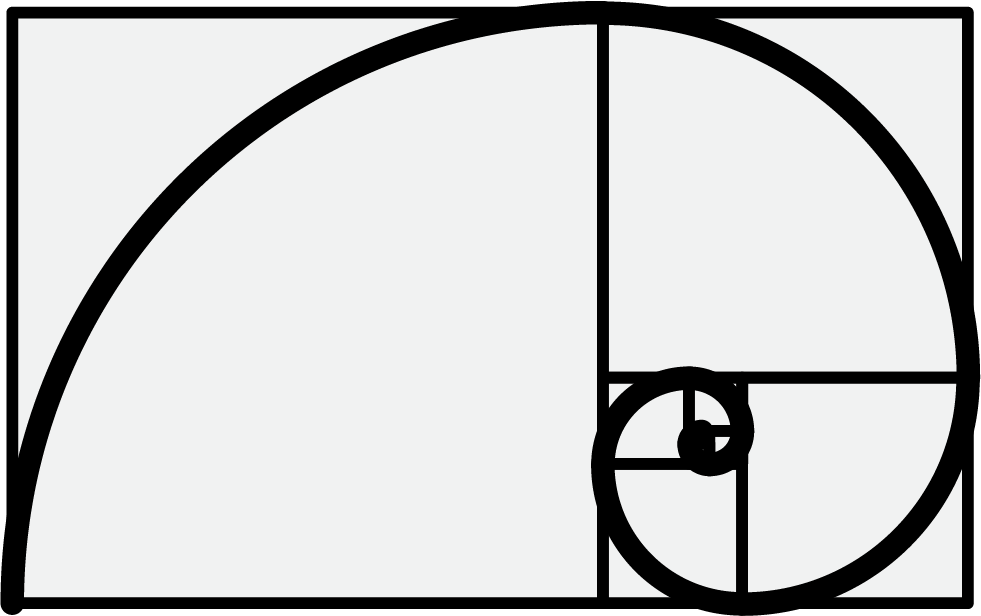
\includegraphics[height=0.75cm]{../../AAA_template_latex_settings/pwr-control_logo_doc.png}}
\lfoot{\href{https://github.com/pwr-control}{\color{black} pwr-control}}
\cfoot{-\ \thepage\ -}
\rfoot{\textit{}}
\renewcommand{\headrulewidth}{0.4pt}
\renewcommand{\footrulewidth}{0.4pt}


\geometry{
	a4paper,
	top    = 2.5cm,
	bottom = 3.0cm,
	left   = 2.5cm,
	right  = 2.5cm
}

\hypersetup{
	colorlinks = true,
	urlcolor   = blue,
	linkcolor  = black,
	citecolor  = black
}

\pagenumbering{gobble}



\usetikzlibrary{decorations.pathreplacing,fit,shapes.geometric}
\usepackage[european,straightvoltages]{circuitikz}
\ctikzset{voltage dir=EF}

\newcommand{\ped}[1]{_{\mathrm{#1}}}
\newcommand{\code}[1]{\texttt{#1}}
\renewcommand{\tabularxcolumn}[1]{>{\raggedright\arraybackslash}p{#1}}
\setlength{\emergencystretch}{3em}
\sisetup{per-mode=symbol}

% ---------------- document metadata (read by the title page) ----------------
\newcommand{\DocCategory}{Technical Note and User Guide}
\newcommand{\DocField}{Power Electronics and Control Systems}

\newcommand{\DocTitle}{%
	{\fontsize{20}{24}\selectfont\bfseries Grid-forming and grid-following AFE blocks} \\[16pt]
	{\fontsize{16}{20}\selectfont\bfseries two-level bridge with LCL filter: description and user guide}
}

\newcommand{\DocSubtitle}{%
	The library blocks \code{grid\_forming\_dqctrl} and \code{grid\_following\_dqctrl} of \code{pwr-control/library}: what they do, how they are built, how to use them. This note is the Help of the two block masks.
}

\newcommand{\DocAuthor}{Davide Bagnara}
\newcommand{\DocRevision}{00}
\newcommand{\DocDate}{October 2026}

\newcommand{\DocAbstract}{%
	The library \code{pwr-control/library} has two three-phase converters that fit in one Simulink block each: \code{grid\_forming\_dqctrl} and \code{grid\_following\_dqctrl}. Both are active front ends (AFE) built on the same power stage, a two-level bridge with a DC-link capacitor and an LCL filter written as one Simscape component, and both carry their whole digital control and PWM in one MATLAB Function. The grid-forming block makes the voltage and the frequency of an island: a free-running phase generator sets the frequency, a voltage loop on the positive sequence of the terminal voltage sets the amplitude, an optional loop cancels the negative-sequence voltage caused by unbalanced loads, and several blocks can feed one load as master and slaves. The grid-following block connects a DC link to an existing grid: a PLL finds the grid angle, a voltage loop keeps the DC link at its reference and a current loop sets the exchanged current. This note describes the two blocks in simple words, with their ports, measurement and gate vectors, parameter structure, control chain and control log, and gives a short user guide with two example parameter files.
}

\newcommand{\RevisionHistory}{%
	00 & October 2026 & First issue: description of the two blocks, user guide, example parameter files. & \DocAuthor \\
}

\newcommand{\MetaLabelA}{Project Repository}
\newcommand{\MetaValueAUrl}{https://github.com/pwr-control/library.git}
\newcommand{\MetaValueALabel}{library.git (masked\_models/grid\_forming, grid\_following)}

\newcommand{\MetaLabelB}{Framework}
\newcommand{\MetaValueB}{MATLAB/Simulink/Simscape}

\begin{document}

% =============================================================
%  pwr-control LaTeX template - FRONTESPIZIO
%
%  Da richiamare come prima istruzione dopo \begin{document}:
%      % =============================================================
%  pwr-control LaTeX template - FRONTESPIZIO
%
%  Da richiamare come prima istruzione dopo \begin{document}:
%      % =============================================================
%  pwr-control LaTeX template - FRONTESPIZIO
%
%  Da richiamare come prima istruzione dopo \begin{document}:
%      \input{../../AAA_template_latex_settings/titlepage}
%
%  Il documento deve definire prima di \begin{document}:
%      \DocCategory   categoria del documento
%      \DocField      area tecnica
%      \DocTitle      titolo (una o due righe)
%      \DocSubtitle   sottotitolo
%      \DocAuthor     autore/i, separati da virgola
%      \DocRevision   numero di revisione corrente (es. 00)
%      \DocDate       data della revisione corrente
%      \DocAbstract   abstract
%      \RevisionHistory  righe della tabella di revisione, nel formato
%                        Rev. & Date & Description & Authors \\
%      \MetaLabelA \MetaValueAUrl \MetaValueALabel
%      \MetaLabelB \MetaValueB
% =============================================================

\providecommand{\DocCategory}{Technical Research Report}
\providecommand{\DocField}{Power Electronics and Control Systems}
\providecommand{\DocSubtitle}{}
\providecommand{\DocRevision}{00}
\providecommand{\DocAbstract}{}
\providecommand{\RevisionHistory}{%
	\DocRevision & \DocDate & First issue. & \DocAuthor \\
}

\titlepage

% ---- Intestazione centrata ----
\begin{center}
	{\Large\scshape \DocCategory}\\[8pt]
	{\large\scshape \DocField}
\end{center}

\vspace{30pt plus 4pt minus 14pt}
\noindent\rule{\linewidth}{0.8pt}

% ---- Titolo ----
\begin{center}
	\DocTitle
\end{center}

\vspace{4pt}
\noindent\rule{\linewidth}{2.2pt}

% ---- Sottotitolo ----
\begin{center}
	\begin{onehalfspace}
		{\large\itshape \DocSubtitle}
	\end{onehalfspace}
\end{center}

% ---- Authors / Revision / Date ----
\vspace{30pt plus 4pt minus 14pt}

\noindent
\begin{minipage}[t]{0.46\linewidth}
	\raggedright
	\textbf{Authors:}\\[2pt]
	\DocAuthor
\end{minipage}%
\hfill
\begin{minipage}[t]{0.22\linewidth}
	\centering
	\textbf{Revision:}\\[2pt]
	\DocRevision
\end{minipage}%
\hfill
\begin{minipage}[t]{0.30\linewidth}
	\raggedleft
	\textbf{Date:}\\[2pt]
	\DocDate
\end{minipage}

\vspace{10pt}
\noindent\rule{\linewidth}{0.8pt}

% ---- Abstract ----
\vspace{24pt plus 4pt minus 12pt}

\begin{center}
	\begin{minipage}{0.88\linewidth}
		\footnotesize
		\begin{onehalfspace}
			\textbf{Abstract:} \DocAbstract
		\end{onehalfspace}
	\end{minipage}
\end{center}

\vfill

% ---- Revision history ----
\begin{center}
	\begin{minipage}{0.96\linewidth}
		\centering
		{\footnotesize\scshape Revision history}\\[6pt]
		{\footnotesize
			\begin{tabular}{@{}cl>{\raggedright\arraybackslash}p{0.36\linewidth}>{\raggedright\arraybackslash}p{0.28\linewidth}@{}}
				\toprule
				\textbf{Rev.} & \textbf{Date} & \textbf{Description} & \textbf{Authors} \\
				\midrule
				\RevisionHistory
				\bottomrule
			\end{tabular}}
	\end{minipage}
\end{center}

\vspace{18pt plus 4pt minus 10pt}

% ---- Metadati in fondo ----
\noindent
\begin{tabular}{@{} r @{\quad} l @{}}
	\textsc{\MetaLabelA:} & {\href{\MetaValueAUrl}{\MetaValueALabel}} \\[3pt]
	\textsc{\MetaLabelB:} & {\MetaValueB}       \\[3pt]
\end{tabular}

% =============================================================
%  Fine frontespizio
% =============================================================
\newpage
\pagenumbering{arabic}
\setcounter{page}{1}

%
%  Il documento deve definire prima di \begin{document}:
%      \DocCategory   categoria del documento
%      \DocField      area tecnica
%      \DocTitle      titolo (una o due righe)
%      \DocSubtitle   sottotitolo
%      \DocAuthor     autore/i, separati da virgola
%      \DocRevision   numero di revisione corrente (es. 00)
%      \DocDate       data della revisione corrente
%      \DocAbstract   abstract
%      \RevisionHistory  righe della tabella di revisione, nel formato
%                        Rev. & Date & Description & Authors \\
%      \MetaLabelA \MetaValueAUrl \MetaValueALabel
%      \MetaLabelB \MetaValueB
% =============================================================

\providecommand{\DocCategory}{Technical Research Report}
\providecommand{\DocField}{Power Electronics and Control Systems}
\providecommand{\DocSubtitle}{}
\providecommand{\DocRevision}{00}
\providecommand{\DocAbstract}{}
\providecommand{\RevisionHistory}{%
	\DocRevision & \DocDate & First issue. & \DocAuthor \\
}

\titlepage

% ---- Intestazione centrata ----
\begin{center}
	{\Large\scshape \DocCategory}\\[8pt]
	{\large\scshape \DocField}
\end{center}

\vspace{30pt plus 4pt minus 14pt}
\noindent\rule{\linewidth}{0.8pt}

% ---- Titolo ----
\begin{center}
	\DocTitle
\end{center}

\vspace{4pt}
\noindent\rule{\linewidth}{2.2pt}

% ---- Sottotitolo ----
\begin{center}
	\begin{onehalfspace}
		{\large\itshape \DocSubtitle}
	\end{onehalfspace}
\end{center}

% ---- Authors / Revision / Date ----
\vspace{30pt plus 4pt minus 14pt}

\noindent
\begin{minipage}[t]{0.46\linewidth}
	\raggedright
	\textbf{Authors:}\\[2pt]
	\DocAuthor
\end{minipage}%
\hfill
\begin{minipage}[t]{0.22\linewidth}
	\centering
	\textbf{Revision:}\\[2pt]
	\DocRevision
\end{minipage}%
\hfill
\begin{minipage}[t]{0.30\linewidth}
	\raggedleft
	\textbf{Date:}\\[2pt]
	\DocDate
\end{minipage}

\vspace{10pt}
\noindent\rule{\linewidth}{0.8pt}

% ---- Abstract ----
\vspace{24pt plus 4pt minus 12pt}

\begin{center}
	\begin{minipage}{0.88\linewidth}
		\footnotesize
		\begin{onehalfspace}
			\textbf{Abstract:} \DocAbstract
		\end{onehalfspace}
	\end{minipage}
\end{center}

\vfill

% ---- Revision history ----
\begin{center}
	\begin{minipage}{0.96\linewidth}
		\centering
		{\footnotesize\scshape Revision history}\\[6pt]
		{\footnotesize
			\begin{tabular}{@{}cl>{\raggedright\arraybackslash}p{0.36\linewidth}>{\raggedright\arraybackslash}p{0.28\linewidth}@{}}
				\toprule
				\textbf{Rev.} & \textbf{Date} & \textbf{Description} & \textbf{Authors} \\
				\midrule
				\RevisionHistory
				\bottomrule
			\end{tabular}}
	\end{minipage}
\end{center}

\vspace{18pt plus 4pt minus 10pt}

% ---- Metadati in fondo ----
\noindent
\begin{tabular}{@{} r @{\quad} l @{}}
	\textsc{\MetaLabelA:} & {\href{\MetaValueAUrl}{\MetaValueALabel}} \\[3pt]
	\textsc{\MetaLabelB:} & {\MetaValueB}       \\[3pt]
\end{tabular}

% =============================================================
%  Fine frontespizio
% =============================================================
\newpage
\pagenumbering{arabic}
\setcounter{page}{1}

%
%  Il documento deve definire prima di \begin{document}:
%      \DocCategory   categoria del documento
%      \DocField      area tecnica
%      \DocTitle      titolo (una o due righe)
%      \DocSubtitle   sottotitolo
%      \DocAuthor     autore/i, separati da virgola
%      \DocRevision   numero di revisione corrente (es. 00)
%      \DocDate       data della revisione corrente
%      \DocAbstract   abstract
%      \RevisionHistory  righe della tabella di revisione, nel formato
%                        Rev. & Date & Description & Authors \\
%      \MetaLabelA \MetaValueAUrl \MetaValueALabel
%      \MetaLabelB \MetaValueB
% =============================================================

\providecommand{\DocCategory}{Technical Research Report}
\providecommand{\DocField}{Power Electronics and Control Systems}
\providecommand{\DocSubtitle}{}
\providecommand{\DocRevision}{00}
\providecommand{\DocAbstract}{}
\providecommand{\RevisionHistory}{%
	\DocRevision & \DocDate & First issue. & \DocAuthor \\
}

\titlepage

% ---- Intestazione centrata ----
\begin{center}
	{\Large\scshape \DocCategory}\\[8pt]
	{\large\scshape \DocField}
\end{center}

\vspace{30pt plus 4pt minus 14pt}
\noindent\rule{\linewidth}{0.8pt}

% ---- Titolo ----
\begin{center}
	\DocTitle
\end{center}

\vspace{4pt}
\noindent\rule{\linewidth}{2.2pt}

% ---- Sottotitolo ----
\begin{center}
	\begin{onehalfspace}
		{\large\itshape \DocSubtitle}
	\end{onehalfspace}
\end{center}

% ---- Authors / Revision / Date ----
\vspace{30pt plus 4pt minus 14pt}

\noindent
\begin{minipage}[t]{0.46\linewidth}
	\raggedright
	\textbf{Authors:}\\[2pt]
	\DocAuthor
\end{minipage}%
\hfill
\begin{minipage}[t]{0.22\linewidth}
	\centering
	\textbf{Revision:}\\[2pt]
	\DocRevision
\end{minipage}%
\hfill
\begin{minipage}[t]{0.30\linewidth}
	\raggedleft
	\textbf{Date:}\\[2pt]
	\DocDate
\end{minipage}

\vspace{10pt}
\noindent\rule{\linewidth}{0.8pt}

% ---- Abstract ----
\vspace{24pt plus 4pt minus 12pt}

\begin{center}
	\begin{minipage}{0.88\linewidth}
		\footnotesize
		\begin{onehalfspace}
			\textbf{Abstract:} \DocAbstract
		\end{onehalfspace}
	\end{minipage}
\end{center}

\vfill

% ---- Revision history ----
\begin{center}
	\begin{minipage}{0.96\linewidth}
		\centering
		{\footnotesize\scshape Revision history}\\[6pt]
		{\footnotesize
			\begin{tabular}{@{}cl>{\raggedright\arraybackslash}p{0.36\linewidth}>{\raggedright\arraybackslash}p{0.28\linewidth}@{}}
				\toprule
				\textbf{Rev.} & \textbf{Date} & \textbf{Description} & \textbf{Authors} \\
				\midrule
				\RevisionHistory
				\bottomrule
			\end{tabular}}
	\end{minipage}
\end{center}

\vspace{18pt plus 4pt minus 10pt}

% ---- Metadati in fondo ----
\noindent
\begin{tabular}{@{} r @{\quad} l @{}}
	\textsc{\MetaLabelA:} & {\href{\MetaValueAUrl}{\MetaValueALabel}} \\[3pt]
	\textsc{\MetaLabelB:} & {\MetaValueB}       \\[3pt]
\end{tabular}

% =============================================================
%  Fine frontespizio
% =============================================================
\newpage
\pagenumbering{arabic}
\setcounter{page}{1}


\tableofcontents
\listoffigures
\listoftables
\newpage

\begin{onehalfspace}

% =============================================================
\section*{Nomenclature}
\addcontentsline{toc}{section}{Nomenclature}
\label{sec:nomenclature}

\rowcolors{2}{tableShade}{white}
\begin{longtable}{@{} l p{0.74\linewidth} @{}}
	\toprule
	\textbf{Symbol} & \textbf{Meaning} \\
	\midrule
	\endfirsthead
	\toprule
	\textbf{Symbol} & \textbf{Meaning} \\
	\midrule
	\endhead
	\bottomrule
	\endfoot
	\bottomrule
	\endlastfoot
	AFE & active front end: a three-phase PWM converter between a DC link and a three-phase AC network, power in both directions \\
	GFM, GFL & grid-forming, grid-following (the two blocks) \\
	pu & per unit: a quantity divided by its base value \\
	$u\ped{bez}$, $i\ped{bez}$ & base voltage (peak of the phase voltage) and base current (peak of the phase current) of the pu system \\
	$u\ped{dc,nom}$ & base of the DC-link voltage \\
	$f\ped{grid}$, $\omega\ped{0}$ & fundamental frequency of the AC side and its angular value $2\pi f\ped{grid}$ \\
	$f\ped{pwm}$, $t\ped{s}$ & PWM frequency and control period ($t\ped{s} = 1/(2 f\ped{pwm})$ with double update) \\
	$t\ped{c}$ & sample time of the block and step of the Simscape local solver \\
	$\alpha\beta$ & stationary two-axis frame (Clarke transform of the three phases) \\
	$\xi\eta$ ($dq$) & rotating two-axis frame, turned by the angle $\theta$; the library calls the axes $\xi$ and $\eta$ \\
	$\theta$, $\gamma$ & angle of the rotating frame: from the phase generator (GFM), from the PLL (GFL) \\
	FHT & first harmonic tracker: a resonant observer that extracts the fundamental of a signal and its quadrature \\
	PLL & phase-locked loop: finds the angle of the grid voltage \\
	TRGO & trigger of the control, raised at the bottom (and top) of the carrier \\
	SVPWM & space vector PWM: turns the voltage reference into the three duties \\
	NSC & negative-sequence compensator of the grid-forming block \\
	$M$, $G$ & measurement vector (14, pu) and gate vector (6, V) of the power stage \\
	$m\ped{d}$, $m\ped{q}$ & outputs of the current loop: the voltage reference in pu of $u\ped{bez}$ (modulation index) \\
	$d\ped{a}$, $d\ped{b}$, $d\ped{c}$ & duties of the three legs on the carrier, between 0 and 1 \\
\end{longtable}
\addtocounter{table}{-1}
\rowcolors{1}{white}{white}

% =============================================================
\section{Introduction}
\label{sec:intro}

An active front end (AFE) is a three-phase PWM converter placed between a DC link and a three-phase AC network. Power can flow in both directions. The same hardware can be run in two ways (Figure~\ref{fig:roles}):

\begin{itemize}[nosep]
	\item \textbf{grid-following}: the AC network already has a voltage and a frequency (the public grid, or another converter that forms it). The converter measures the grid voltage, finds its angle with a phase-locked loop (PLL) and injects a controlled current. It regulates its own DC-link voltage, so the active power follows what the DC side takes or gives;
	\item \textbf{grid-forming}: there is no grid. The converter itself creates the three-phase voltage, with a fixed frequency and a fixed amplitude, like a generator feeding an island. It needs a DC source, for instance a battery, able to supply the power that the loads take.
\end{itemize}

\begin{figure}[H]
	\centering
	\begin{tikzpicture}[font=\footnotesize, >=Latex, node distance=0.7cm,
		blk/.style={draw, thick, rounded corners=2pt, minimum height=1.15cm, align=center, fill=orange!15},
		src/.style={draw, thick, rounded corners=2pt, minimum height=1.15cm, minimum width=2.9cm, align=center, fill=gray!10}]
		\node[src] (dc1) {DC side\\load or source};
		\node[blk, right=of dc1] (afe1) {\code{grid\_following\_dqctrl}\\PLL, DC-link loop, current loop};
		\node[src, right=of afe1] (grid) {existing grid\\voltage and frequency given};
		\draw[<->, thick] (dc1) -- (afe1);
		\draw[<->, thick] (afe1) -- (grid);
		\node[above=3pt of afe1, font=\small\bfseries] {(a) grid-following};
		\node[src, below=1.7cm of dc1] (bat) {battery\\supplies the power};
		\node[blk, right=of bat] (afe2) {\code{grid\_forming\_dqctrl}\\phase generator, voltage loop,\\current loop};
		\node[src, right=1.5cm of afe2] (isl) {island\\transformer and loads};
		\draw[<->, thick] (bat) -- (afe2);
		\draw[->, thick] (afe2) -- (isl) node[midway, above=1pt, font=\scriptsize] {forms $u$, $f$};
		\node[above=3pt of afe2, font=\small\bfseries] {(b) grid-forming};
	\end{tikzpicture}
	\captionsetup{width=0.85\textwidth, font=small}
	\caption[The two roles of an AFE.]{The two roles of an AFE and the block of the library for each of them.}
	\label{fig:roles}
\end{figure}

The library has one block for each role. Both blocks have the same power stage, the same acquisition of the measurements, the same current loop and the same PWM. They differ in what sets the angle of the rotating frame and in what sets the current references: a free-running phase generator and a voltage loop in the grid-forming block, a PLL and a DC-link voltage loop in the grid-following one.

Each converter is \emph{one} Simulink block, with two nonvirtual blocks inside: the power stage is a Simscape language component and the whole control is a MATLAB Function. The reason is the MATLAB Home licence used for the project, which allows at most 1000 nonvirtual blocks per model, referenced models and library links included. A converter built with the discrete blocks of the library costs several hundred of them; one of these blocks costs a handful, so a model can hold many converters, for instance two grid-forming converters in parallel on one transformer, or a grid-forming converter feeding grid-following ones.

The two blocks were built from two Simulink study models made with the discrete blocks of the library, \code{grid\_forming\_dq.slx} of \code{pwr-control/modelization-and-control} (\SI{400}{\volt}, \SI{250}{\kilo\watt}, \SI{50}{\hertz}, an unbalanced load on a Dyn11 transformer) and \code{grid\_follower\_dq.slx}: the MATLAB Functions reproduce those models block by block, and the headers of the sources say which block of the model each line comes from. The files are in \code{pwr-control/library} \cite{library_repo}:

\begin{itemize}[nosep]
	\item \path{library/masked_models/grid_forming/grid_forming_dqctrl.slx}, block \code{grid\_forming\_dqctrl\_mod1}; the control source is \path{grid_forming/private/afe_dq_ctrl_pwm.m} and \path{grid_forming/update_grid_forming_dqctrl.m} loads it into the block;
	\item \path{library/masked_models/grid_following/grid_following_dqctrl.slx}, block \code{grid\_following\_dqctrl\_mod1}; the control source is inside the block (MATLAB Function \code{afe\_dq\_follower\_ctrl\_pwm});
	\item \path{library/foundation/pwr_electronics/+afe_ssc/afe_two_level_lcl.ssc}, the Simscape component of the power stage, compiled into \path{afe_ssc_lib.slx}.
\end{itemize}

This note describes the blocks and tells how to use them. It does not repeat the design of the control loops: the structure of the grid-forming controller, the analysis of every loop and the choice of the discretization are in \cite{gfm_note}, and the background on grid converters is in \cite{teodorescu2011}. Section~\ref{sec:quickstart} is the user guide. Section~\ref{sec:power_stage} describes the power stage, Section~\ref{sec:common} the parts of the control that the two blocks share, Sections~\ref{sec:gfm} and~\ref{sec:gfl} the two blocks one by one, Section~\ref{sec:param} the parameter structure and Section~\ref{sec:limits} what the blocks do not model.

% =============================================================
\section{Quick start: how to use the blocks}
\label{sec:quickstart}

\subsection{What you need}
\label{sec:need}

\begin{itemize}[nosep]
	\item MATLAB with Simulink, Simscape and Simscape Electrical (R2026b was used to save the blocks).
	\item The repository \code{pwr-control/library} on the MATLAB path \emph{with subfolders}.
	\item The compiled Simscape library \path{library/foundation/pwr_electronics/afe_ssc_lib.slx}. It is in the repository. Rebuild it only after an edit of the \code{.ssc} source:
	\begin{center}
		\code{cd library/foundation/pwr\_electronics} \quad then \quad \code{ssc\_build afe\_ssc}
	\end{center}
\end{itemize}

\subsection{Put a block in a model, step by step}
\label{sec:steps}

\begin{enumerate}[nosep]
	\item \textbf{Drag the block.} Open \code{grid\_forming\_dqctrl.slx} or \code{grid\_following\_dqctrl.slx} and drag the block into your model. The copy stays a library link, so an update of the library updates the model. Figure~\ref{fig:minimal} shows the smallest useful model for each block.
	\item \textbf{Connect the AC side.} The three physical ports \code{ug\_a}, \code{ug\_b}, \code{ug\_c} on the left are the terminals \emph{after} the LCL filter. Connect them to the three-phase network: for the grid-forming block the load (a transformer and its loads, or a three-phase RL load), for the grid-following block the grid (an ideal three-phase source with a series impedance, or the grid emulator of the library).
	\item \textbf{Connect the DC side.} The two physical ports \code{Udc(+)} and \code{Udc($-$)} on the right are the DC link. The DC-link capacitor is \emph{inside} the block. Connect a DC source with a series resistance (a battery, or a DC Voltage Source with a resistor of a few tens of \si{\milli\ohm}), or the DC load of the grid-following converter. The capacitor starts discharged, so a source without any series resistance gives a very large current at the first step.
	\item \textbf{Simscape housekeeping.} The network needs one Electrical Reference (for instance on \code{Udc($-$)} or on the star point of the AC source) and one Solver Configuration block. Use the local solver with a fixed step equal to \code{p.pwm.tc}, Backward Euler, two or three nonlinear iterations, as in the study models. The global solver can be a variable-step one (\code{ode23tb}) with the maximum step set to the same value.
	\item \textbf{Connect \code{t\_master}.} This Simulink input is the master time of the model: a Clock block is enough. In the models that have a global timing subsystem, connect its master time instead.
	\item \textbf{Build the parameter structure.} The mask has one parameter, the structure \code{p} with the three fields \code{p.hw}, \code{p.pwm} and \code{p.ctrl} (Section~\ref{sec:param}). Two example files give a complete structure for a \SI{400}{\volt}, \SI{250}{\kilo\watt}, \SI{50}{\hertz} converter switching at \SI{4}{\kilo\hertz}:
	\begin{center}
		\code{p = grid\_forming\_param\_example();} \qquad \code{p = grid\_following\_param\_example();}
	\end{center}
	Type \code{p} in the mask, or the name of your own structure (the study models use \code{param.afe\_mod(1)} and \code{param.afe\_follower(1)}). For another converter, copy the example file next to your model, change the numbers and keep the field names.
	\item \textbf{Grid-forming only: the \code{sync} ports.} A master ignores the input \code{sync}: connect a Ground block to it and a Terminator to \code{sync\_out}, so that Simulink does not warn about unconnected ports. For converters in parallel, connect \code{sync\_out} of the master to \code{sync} of every slave and set \code{p.ctrl.slave = 1} in the slaves (Section~\ref{sec:master_slave}).
	\item \textbf{Run and look at the outputs.} The output \code{m} is the measurement vector of the power stage (14 values in pu, Table~\ref{tab:meas}); \code{ctrl\_log} is the control log (43 or 45 values, Tables~\ref{tab:log_gfm} and~\ref{tab:log_gfl}). Log them with To Workspace blocks and plot them with the indices of the tables.
\end{enumerate}

\begin{figure}[H]
	\centering
	\begin{tikzpicture}[font=\scriptsize, >=Latex,
		blk/.style={draw, thick, rounded corners=2pt, align=center, fill=orange!15, minimum height=1.9cm, minimum width=3.6cm},
		el/.style={draw, thick, align=center, fill=gray!10, minimum height=0.8cm, minimum width=2.3cm},
		sl/.style={draw, thick, align=center, fill=blue!6, minimum height=0.55cm, minimum width=1.5cm},
		ref/.style={draw, thick, align=center, fill=white, minimum height=0.55cm}]
		% (a) grid-forming
		\node[blk] (gfm) at (0,0) {\code{grid\_forming\_dqctrl\_mod1}\\[2pt]mask: \code{p}};
		\node[el] (load) at (-5.4,0.5) {three-phase\\RL load};
		\node[el] (bat) at (5.4,0.5) {DC source\\$+$ series $R$};
		\node[sl] (clk) at (-5.4,-0.4) {Clock};
		\node[sl] (gnd) at (-5.4,-1.3) {Ground};
		\node[ref] (er) at (5.4,-1.0) {Electrical Reference};
		\node[ref] (sc) at (5.4,-2.0) {Solver Configuration\\local solver, step \code{p.pwm.tc}};
		\node[sl] (term) at (5.4,-3.1) {Terminator};
		\draw[thick] (load.east) -- (gfm.west |- load.east) node[midway, above] {ug\_a/b/c};
		\draw[thick] (gfm.east |- bat.west) -- (bat.west) node[midway, above] {Udc(+)/($-$)};
		\draw[->, thick] (clk.east) -- (gfm.west |- clk.east) node[midway, above] {t\_master};
		\draw[->, thick] (gnd.east) -- (gfm.west |- gnd.east) node[midway, above] {sync};
		\draw[->, thick] ([yshift=-0.6cm]gfm.east) -- ++(0.7,0) |- (term.west);
		\node[above right] at ([yshift=-0.6cm]gfm.east) {sync\_out};
		\draw[thick] (er.north) -- (bat.south);
		\draw[thick] (sc.north) -- (er.south);
		\node[font=\small\bfseries] at (0,1.55) {(a) grid-forming: the block feeds a load};
		% (b) grid-following
		\node[blk] (gfl) at (0,-5.7) {\code{grid\_following\_dqctrl\_mod1}\\[2pt]mask: \code{p}};
		\node[el] (grid) at (-5.4,-5.2) {three-phase source\\$+$ series $L$ (grid)};
		\node[el] (dcl) at (5.4,-5.2) {DC load or source\\resistor, current source};
		\node[sl] (clk2) at (-5.4,-6.1) {Clock};
		\node[ref] (er2) at (5.4,-6.7) {Electrical Reference};
		\node[ref] (sc2) at (5.4,-7.7) {Solver Configuration\\local solver, step \code{p.pwm.tc}};
		\draw[thick] (grid.east) -- (gfl.west |- grid.east) node[midway, above] {ug\_a/b/c};
		\draw[thick] (gfl.east |- dcl.west) -- (dcl.west) node[midway, above] {Udc(+)/($-$)};
		\draw[->, thick] (clk2.east) -- (gfl.west |- clk2.east) node[midway, above] {t\_master};
		\draw[thick] (er2.north) -- (dcl.south);
		\draw[thick] (sc2.north) -- (er2.south);
		\node[font=\small\bfseries] at (0,-4.15) {(b) grid-following: the block hangs on a grid};
	\end{tikzpicture}
	\captionsetup{width=0.88\textwidth, font=small}
	\caption[Minimal test models.]{Minimal test models for the two blocks. The outputs \code{m} and \code{ctrl\_log} (not drawn) go to To Workspace blocks or Scopes. The DC-link capacitor and the LCL filter are inside the block.}
	\label{fig:minimal}
\end{figure}

\subsection{Things to check before the first run}
\label{sec:checks}

\begin{mybox}
\begin{itemize}[nosep]
	\item \code{p.pwm.tc} must be the step of the Simscape local solver: the MATLAB Function and the Unit Delay of the measurements run at this sample time\footnote{Up to October 2026 the Unit Delay of the two blocks read \code{param.glb\_time.tc} from the base workspace; it now reads \code{p.pwm.tc}, like the other single-block converters of the library. A model that still defines \code{param.glb\_time.tc} keeps working.}, and the gates are read by Simscape at the solver step. The example files use $t\ped{s}/200$, that is \SI{0.625}{\micro\second} at \SI{4}{\kilo\hertz} with double update.
	\item \code{p.ctrl.ts} must be the control period: $1/(2 f\ped{pwm})$ with \code{p.pwm.double\_update = 1}, $1/f\ped{pwm}$ otherwise. \code{p.ctrl.ts\_int} (sample time of the PI integrators) is normally the same value.
	\item \code{p.hw.ubez}, \code{p.hw.ibez} and \code{p.hw.udc\_nom} are the bases of every pu quantity: the measurements, the references and the limits. Check them first when a loop behaves strangely.
	\item There is no soft start and no pre-charge in the blocks. The grid-forming block applies its voltage reference from the first trigger; the grid-following block charges its DC link through the bridge diodes as soon as the grid voltage is present, and its DC-link reference steps at \code{p.ctrl.udc\_t\_step} through a low-pass filter. Expect a transient in the first grid periods.
	\item The first harmonic tracker is held at zero while $t <$ \code{p.ctrl.fht\_t\_reset}. Keep this time short (a few control periods).
	\item The structure \code{p} must exist in the base workspace (or in the model workspace) when the model is updated: run the example file, or your initialization script, first.
	\item Grid-forming, converters in parallel: master and slaves need the same \code{p.ctrl.k\_time}, the same carrier phase \code{p.pwm.phase}, the same \code{p.pwm.double\_update} and the same \code{p.ctrl.nsc\_enable}.
\end{itemize}
\end{mybox}

\subsection{Reading the results}
\label{sec:results}

In the control log, \code{trgo} (index 3) toggles twice per PWM period and the three duties (indices 31 to 33 of the grid-forming log, 38 to 40 of the grid-following one) stay between \code{p.pwm.m\_low} and \code{p.pwm.m\_up} when the converter is not saturated. The clip flag of the current loop (\code{clip\_i}) is 0 in normal operation; a clip flag that stays at 1 means that the voltage reference asks more than the DC link can give. For the grid-forming block, $u\ped{\xi}$ (index 19) settles at \code{p.ctrl.ug\_ref} and $u\ped{\eta}$ (index 20) at zero in a few tens of milliseconds; for the grid-following block, \code{omega\_pll\_pu} (index 6) settles at 1 when the PLL is locked and \code{udc} (index 16) follows \code{udc\_ref} (index 24). All currents and voltages of \code{m} and of the log are in pu of \code{p.hw.ibez}, \code{p.hw.ubez} and \code{p.hw.udc\_nom}.

% =============================================================
\section{The power stage: \code{afe\_ssc.afe\_two\_level\_lcl}}
\label{sec:power_stage}

\subsection{Circuit}
\label{sec:circuit}

The power stage is one Simscape language component (Figure~\ref{fig:circuit}): a three-phase two-level bridge, a DC-link capacitor and an LCL filter. The bridge has six switches, each with an antiparallel diode. The DC link is a capacitor $C\ped{dc}$ with its series resistance $R\ped{dc}$ between \code{Udc(+)} and \code{Udc($-$)}. The filter has a converter-side three-phase inductor ($L\ped{1}$, $R\ped{1}$), three capacitors $C\ped{f}$ in star with a series resistance $R\ped{cf}$ each and a floating star point, and a grid-side three-phase inductor ($L\ped{2}$, $R\ped{2}$). The terminals \code{ug\_a}, \code{ug\_b}, \code{ug\_c} are the grid side of $L\ped{2}$.

\begin{figure}[H]
	\centering
	\ctikzset{transistors/scale=0.8, bipoles/length=1.0cm}
	\begin{subfigure}[b]{\textwidth}
		\centering
		\begin{circuitikz}[european, font=\scriptsize, scale=0.85, transform shape]
			\draw (0,3) -- (7.9,3) node[right] {Udc(+)};
			\draw (0,-3) -- (7.9,-3) node[right] {Udc($-$)};
			\draw (0.5,3) to[R, l_=$R\ped{dc}$] (0.5,1.0) to[C, l_=$C\ped{dc}$] (0.5,-3);
			\foreach \x/\ph/\ym in {1.8/a/0.6, 4.1/b/0, 6.4/c/-0.6} {
				\draw (\x,3) to[Tnigbt, l_=$\ph^{+}$] (\x,\ym) to[Tnigbt, l_=$\ph^{-}$] (\x,-3);
				\draw (\x+0.95,\ym) to[D] (\x+0.95,3);
				\draw (\x+0.95,-3) to[D] (\x+0.95,\ym);
				\draw (\x,\ym) -- (7.9,\ym) node[right] {$\ph$};
				\fill (\x,\ym) circle (1.2pt);
				\fill (\x+0.95,\ym) circle (1.2pt);
				\fill (\x,3) circle (1.2pt);
				\fill (\x+0.95,3) circle (1.2pt);
				\fill (\x,-3) circle (1.2pt);
				\fill (\x+0.95,-3) circle (1.2pt);
			}
			\fill (0.5,3) circle (1.2pt);
			\fill (0.5,-3) circle (1.2pt);
		\end{circuitikz}
		\caption{bridge and DC link}
		\label{fig:bridge}
	\end{subfigure}

	\vspace{0.6em}
	\begin{subfigure}[b]{\textwidth}
		\centering
		\begin{circuitikz}[european, font=\scriptsize]
			\draw (0,0) node[left] {$k$} to[R, l=$R\ped{1}$, i_=$i_{1k}$] (1.8,0) to[L, l=$L\ped{1}$] (3.4,0) -- (4.2,0) to[R, l=$R\ped{2}$, i_=$i_{2k}$] (6.0,0) to[L, l=$L\ped{2}$] (7.6,0) -- (8.2,0) node[right] {ug\_$k$};
			\draw (4.2,0) to[R, l_=$R\ped{cf}$] (4.2,-1.6) to[C, l_=$C\ped{f}$] (4.2,-3.0) node[below] {$n$ (floating star point)};
			\fill (4.2,0) circle (1.2pt);
			\draw[->, thick] (4.9,-0.4) -- (4.9,-2.6) node[midway, right] {$u_{ck}$};
		\end{circuitikz}
		\caption{LCL filter, one of the three phases}
		\label{fig:lcl}
	\end{subfigure}
	\captionsetup{width=0.9\textwidth, font=small}
	\caption[Power stage of the blocks.]{Power stage of the two blocks, the Simscape component \code{afe\_ssc.afe\_two\_level\_lcl}. (a) Two-level bridge with the antiparallel diodes and the DC-link capacitor; $a$, $b$, $c$ are the leg midpoints. (b) The LCL filter of one phase $k$: the three capacitor branches meet at the floating star point $n$. The measured quantities are the converter current $i_{1k}$, the capacitor voltage $u_{ck}$, the grid current $i_{2k}$ and the terminal voltage.}
	\label{fig:circuit}
\end{figure}

\subsection{Switch model}
\label{sec:switch}

The switches are numerical, with no losses and no thermal model. A switch with its diode behaves as follows (voltage $v$ from collector to emitter, current $i$ in the same direction): with the gate on ($G > V\ped{th}$) it conducts in both directions through $R\ped{on}$; with the gate off and $v < 0$ the antiparallel diode conducts, again through $R\ped{on}$; with the gate off and $v \ge 0$ it blocks, with the small conductance $G\ped{off}$. There is no dead time and no interlock inside the component: the dead time is made by the control (Section~\ref{sec:gates}), and if both switches of a leg are on the leg shorts the DC link through $2 R\ped{on}$. The gate levels of the example files are \SI{15}{\volt} on and \SI{-10}{\volt} off, against $V\ped{th} = \SI{2.5}{\volt}$.

\subsection{LCL filter}
\label{sec:lcl_eq}

Each three-phase inductor uses the equations of the \code{threephase\_inductor} block of the library: a positive-sequence inductance $L\ped{p}$, a zero-sequence inductance $L\ped{0}$ (the inductance seen by a current that is equal in the three phases), a leakage inductance $L\ped{ls}$ and a series resistance $R$. With $L\ped{m} = (L\ped{p} - L\ped{0})/3$ and $L\ped{a} = (L\ped{0} + L\ped{p} + L\ped{m})/2$, the voltage of phase $x$ is
\begin{equation}
	u_{1x} - u_{2x} = R\, i_x + (L\ped{ls} + L\ped{a})\, \frac{\mathrm{d} i_x}{\mathrm{d} t} - L\ped{m} \left( \frac{\mathrm{d} i_y}{\mathrm{d} t} + \frac{\mathrm{d} i_z}{\mathrm{d} t} \right),
	\label{eq:inductor}
\end{equation}
so the positive sequence sees $L\ped{p} + L\ped{ls}$ and the zero sequence $L\ped{0} + L\ped{ls}$. With $L\ped{0} = L\ped{p}$, the default of the example files, the three phases are independent. The star point of the capacitors is floating, so the three capacitor currents sum to zero. The resonance of the filter with a stiff grid is
\begin{equation}
	f\ped{res} = \frac{1}{2\pi} \sqrt{\frac{L\ped{1} + L\ped{2}}{L\ped{1} L\ped{2} C\ped{f}}},
	\label{eq:fres}
\end{equation}
\SI{1045}{\hertz} with the values of the example files (\SI{330}{\micro\henry}, \SI{360}{\micro\farad}, \SI{80}{\micro\henry}). The current loop damps this resonance only when $f\ped{res}$ is below one sixth of the control frequency, \SI{1333}{\hertz} at \SI{8}{\kilo\hertz} \cite{parker2014}; above it, only $R\ped{cf}$ holds the mode. The initialization script of the study model prints this check.

\subsection{Measurements, gates and bases}
\label{sec:meas}

The component gives its measurements as one physical-signal vector $M$ of 14 values in pu (Table~\ref{tab:meas}) and takes its gate commands as one physical-signal vector $G$ of six voltages (Table~\ref{tab:gates}). The bases are three parameters of the component: $u\ped{bez}$, the peak of the rated phase voltage ($U\ped{nom} \sqrt{2/3}$, \SI{326.6}{\volt} for \SI{400}{\volt}); $i\ped{bez}$, the peak of the rated phase current ($I\ped{nom} \sqrt{2}$, \SI{566.7}{\ampere} for \SI{250}{\kilo\watt} at \SI{400}{\volt} and $\cos\varphi = 0.9$); and $u\ped{dc,nom}$, the rated DC-link voltage (\SI{660}{\volt}). A phase voltage of amplitude $u\ped{bez}$ reads 1 in $M$; a current of amplitude $i\ped{bez}$ reads 1. These are the same bases used by the control for its references and limits.

\begin{table}[H]
	\centering
	\captionsetup{width=0.9\textwidth, font=small}
	\caption[Measurement vector of the power stage.]{Measurement vector $M$ (output \code{m} of the block, 14 pu values). The control reads it one $t\ped{c}$ behind.}
	\label{tab:meas}
	\rowcolors{2}{tableShade}{white}
	\begin{tabularx}{0.95\textwidth}{@{} c l X @{}}
		\toprule
		\textbf{Index} & \textbf{Signal} & \textbf{Meaning and sign} \\
		\midrule
		1, 2, 3 & $i_{1a}$, $i_{1b}$, $i_{1c}$ & converter currents (converter-side inductor), positive \emph{out} of the bridge; the control calls them $i\ped{s}$ \\
		4, 5, 6 & $u_{ca}$, $u_{cb}$, $u_{cc}$ & filter capacitor voltages, capacitor node to star point \\
		7, 8, 9 & $i_{2a}$, $i_{2b}$, $i_{2c}$ & grid currents (grid-side inductor), positive \emph{towards} the terminals; the control calls them $i\ped{g}$ \\
		10, 11, 12 & $u_{ga}$, $u_{gb}$, $u_{gc}$ & terminal voltages without their zero sequence, $u_{ga} = (2 v_a - v_b - v_c)/3$, as a line-to-line sensor would give \\
		13 & $v\ped{dc}$ & DC-link voltage, \code{Udc(+)} minus \code{Udc($-$)}, in pu of $u\ped{dc,nom}$ \\
		14 & $i\ped{c}$ & current of the DC-link capacitor, positive from \code{Udc(+)} to \code{Udc($-$)} \\
		\bottomrule
	\end{tabularx}
	\rowcolors{1}{white}{white}
\end{table}

\begin{table}[H]
	\centering
	\captionsetup{width=0.9\textwidth, font=small}
	\caption[Gate vector of the power stage.]{Gate vector $G$ (six voltages, \code{p.pwm.gate\_on} / \code{p.pwm.gate\_off}).}
	\label{tab:gates}
	\rowcolors{2}{tableShade}{white}
	\begin{tabularx}{0.95\textwidth}{@{} c l X @{}}
		\toprule
		\textbf{Index} & \textbf{Switch} & \textbf{Position} \\
		\midrule
		1, 2 & $a^{+}$, $a^{-}$ & leg a, upper switch (\code{Udc(+)} to midpoint) and lower switch (midpoint to \code{Udc($-$)}) \\
		3, 4 & $b^{+}$, $b^{-}$ & leg b \\
		5, 6 & $c^{+}$, $c^{-}$ & leg c \\
		\bottomrule
	\end{tabularx}
	\rowcolors{1}{white}{white}
\end{table}

\subsection{How the block is assembled}
\label{sec:assembly}

Figure~\ref{fig:block} shows the inside of the two masked blocks. Besides the Simscape component and the MATLAB Function there are only the converters between the two domains: \code{gates}, a Simulink-PS Converter for the six gate voltages; \code{meas}, a PS-Simulink Converter for the 14 measurements, which also feeds the output \code{m}; and \code{meas\_delay}, a Unit Delay of one $t\ped{c}$ on the measurements read by the control, which breaks the algebraic loop between measurements and gates. The parameters of the Simscape component are wired to the fields of \code{p.hw} with the same names; the option of the DC-link capacitor is fixed to \emph{on}.

\begin{figure}[H]
	\centering
	\begin{tikzpicture}[font=\footnotesize, >=Latex,
		ssc/.style={draw, thick, fill=orange!12, minimum height=2.3cm, minimum width=6.6cm, align=center, rounded corners=2pt},
		mf/.style={draw, thick, fill=blue!8, minimum height=2.0cm, minimum width=4.8cm, align=center, rounded corners=2pt},
		cv/.style={draw, thick, fill=gray!10, minimum height=0.8cm, minimum width=2.0cm, align=center},
		port/.style={draw, thick, fill=white, inner sep=2pt, font=\scriptsize}]
		\node[ssc] (ssc) at (0,0) {\code{afe\_ssc.afe\_two\_level\_lcl}\\Simscape component\\two-level bridge, DC-link capacitor,\\LCL filter, 14 measurements};
		\node[cv] (gates) at (-2.2,-2.6) {\code{gates}\\Simulink-PS};
		\node[cv] (meas) at (3.1,-2.6) {\code{meas}\\PS-Simulink};
		\node[cv] (delay) at (3.1,-4.4) {\code{meas\_delay}\\$z^{-1}$ at $t\ped{c}$};
		\node[mf] (ctrl) at (-2.8,-5.0) {\code{afe\_dq\_forming\_ctrl\_pwm} or\\\code{afe\_dq\_follower\_ctrl\_pwm}\\MATLAB Function at $t\ped{c}$\\clock, carrier, control, SVPWM, gates};
		\draw[->, thick] (gates.north) -- (gates.north |- ssc.south) node[midway, right] {$G$ [6] V};
		\draw[->, thick] (meas.north |- ssc.south) -- (meas.north) node[midway, right] {$M$ [14] pu};
		\draw[->, thick] (meas.south) -- (delay.north);
		\draw[->, thick] (delay.west) -- (delay.west -| ctrl.east) node[midway, above, align=center, font=\scriptsize, inner sep=1.5pt] {$M$\\one $t\ped{c}$ behind};
		\draw[->, thick] (ctrl.north) -- (ctrl.north |- gates.south) node[midway, left] {$G$};
		\node[port] (ua) at (-5.0,0.8) {ug\_a};
		\node[port] (ub) at (-5.0,0.0) {ug\_b};
		\node[port] (uc) at (-5.0,-0.8) {ug\_c};
		\node[port] (dcp) at (5.0,0.6) {Udc(+)};
		\node[port] (dcm) at (5.0,-0.6) {Udc($-$)};
		\draw[thick] (ua) -- (ua -| ssc.west);
		\draw[thick] (ub) -- (ub -| ssc.west);
		\draw[thick] (uc) -- (uc -| ssc.west);
		\draw[thick] (dcp) -- (dcp -| ssc.east);
		\draw[thick] (dcm) -- (dcm -| ssc.east);
		\node[port] (tm) at (-6.7,-4.6) {t\_master};
		\draw[->, thick] (tm) -- (tm -| ctrl.west);
		\node[port] (sy) at (-6.7,-5.4) {sync (GFM)};
		\draw[->, thick] (sy) -- (sy -| ctrl.west);
		\node[port] (m) at (5.7,-2.6) {m [14]};
		\draw[->, thick] (meas.east) -- (m);
		\node[port] (log) at (4.6,-5.3) {ctrl\_log [43 / 45]};
		\draw[->, thick] (ctrl.east |- log) -- (log);
		\node[port] (so) at (4.6,-5.9) {sync\_out (GFM)};
		\draw[->, thick] (ctrl.east |- so) -- (so);
		\node[font=\footnotesize, align=center] at (0,1.85) {\code{grid\_forming\_dqctrl\_mod1} / \code{grid\_following\_dqctrl\_mod1}\\mask parameter \code{p} (\code{p.hw}, \code{p.pwm}, \code{p.ctrl})};
	\end{tikzpicture}
	\captionsetup{width=0.85\textwidth, font=small}
	\caption[Structure of the blocks.]{Structure of the two blocks: one Simscape component for the power stage, one MATLAB Function for the control and the PWM, the two domain converters and the one-step delay of the measurements. The \code{sync} ports exist in the grid-forming block only.}
	\label{fig:block}
\end{figure}

% =============================================================
\section{The control: parts common to both blocks}
\label{sec:common}

The MATLAB Function runs at every step $t\ped{c}$. At every step it computes the local clock, the carrier, the trigger flag and the gate commands. The control itself, from the acquisitions to the duties, runs only on the rising edge of the trigger, exactly as the triggered subsystem of the study models. Figure~\ref{fig:timing} shows one PWM period.

\begin{figure}[H]
	\centering
	\begin{tikzpicture}[font=\scriptsize, >=Latex, x=1.75cm, y=1.3cm]
		\fill[gray!20] (0,0.56) rectangle (4.5,0.68);
		\draw[->] (-0.2,0) -- (4.75,0) node[right] {$t$};
		\draw[->] (0,-0.05) -- (0,1.3) node[above] {carrier};
		\draw[thick] (0,0) -- (1,1) -- (2,0) -- (3,1) -- (4,0) -- (4.5,0.5);
		\draw[dashed] (0,0.62) -- (4.5,0.62) node[right] {$d_k$};
		\node[right, gray!60!black] at (4.5,0.78) {$d_k \pm t\ped{d} f\ped{pwm}$};
		\node[left] at (0,1) {1};
		\node[left] at (0,0) {0};
		\foreach \x in {0,1,2,3,4} { \draw[red, very thick] (\x,-0.06) -- (\x,0.1); }
		\node[red, below] at (2,-0.08) {TRGO (double update: bottom and top of the carrier)};
		\draw[<->] (0,1.18) -- (2,1.18) node[midway, above] {$1/f\ped{pwm}$};
		\draw[<->] (2,1.18) -- (3,1.18) node[midway, above] {$t\ped{s}$};
		% upper switch
		\draw[thick, blue!70!black] (0,-0.8) -- (0.68,-0.8) -- (0.68,-0.55) -- (1.32,-0.55) -- (1.32,-0.8) -- (2.68,-0.8) -- (2.68,-0.55) -- (3.32,-0.55) -- (3.32,-0.8) -- (4.5,-0.8);
		\node[left, blue!70!black] at (0,-0.65) {$k^{+}$ on};
		% lower switch
		\draw[thick, green!50!black] (0,-1.1) -- (0.56,-1.1) -- (0.56,-1.35) -- (1.44,-1.35) -- (1.44,-1.1) -- (2.56,-1.1) -- (2.56,-1.35) -- (3.44,-1.35) -- (3.44,-1.1) -- (4.5,-1.1);
		\node[left, green!50!black] at (0,-1.22) {$k^{-}$ on};
		\draw[decorate, decoration={brace, amplitude=4pt}] (2.02,-1.6) -- (2.98,-1.6) node[midway, below=3pt, align=center] {the duties computed at this TRGO,\\from the samples of the previous one,\\are used until the next TRGO};
	\end{tikzpicture}
	\captionsetup{width=0.88\textwidth, font=small}
	\caption[Carrier, trigger and gates.]{Carrier, trigger and gate commands of one leg. The upper switch is on while the carrier is above $d_k + t\ped{d} f\ped{pwm}$, the lower one while it is below $d_k - t\ped{d} f\ped{pwm}$: the grey band is the dead time. With double update the control runs at both ends of the carrier.}
	\label{fig:timing}
\end{figure}

\subsection{Local clock, carrier and trigger}
\label{sec:clock}

The block has a local time $t\ped{loc} = t\ped{master}\, k\ped{time}\, (1 + \mathrm{corr})$. The factor \code{p.ctrl.k\_time} models a converter clock that runs faster or slower than the master clock (1 for an ideal clock), and $\mathrm{corr}$ is the output of a small alignment PI (\code{kp\_align}, \code{ki\_align}, limits \code{lim\_up\_align}, \code{lim\_down\_align}) that pulls the local time back to the master time, as the synchronization of real converters does. The carrier is a triangle between 0 and 1 at $f\ped{pwm}$, shifted by the phase \code{p.pwm.phase}:
\begin{equation}
	\mathrm{ramp} = \frac{1}{\pi} \arcsin\!\big(\sin(2\pi f\ped{pwm} t\ped{loc} - \mathrm{phase} - \pi/2)\big) + \frac{1}{2}.
	\label{eq:ramp}
\end{equation}
The trigger TRGO is raised while the carrier is within $2 f\ped{pwm} t\ped{c}$ of its bottom, and also of its top when \code{p.pwm.double\_update} is 1; the control runs on its rising edge, so once per period or twice per period ($t\ped{s} = 1/f\ped{pwm}$ or $1/(2 f\ped{pwm})$). There is no trigger at the very first evaluation, as with the Trigger block of the models.

\subsection{Acquisitions}
\label{sec:acq}

At every trigger the control samples the terminal voltages $u\ped{g}$, the converter currents $i\ped{s}$, the grid currents $i\ped{g}$ (with the sign changed, so that they are positive out of the converter like $i\ped{s}$) and the DC-link voltage, all from $M$. Each sample is quantized with the step \code{p.ctrl.adc\_q} ($2^{-11}$ pu in the example files, a 12-bit converter on a $\pm 1$ pu scale) and stored; the control of \emph{this} trigger works with the samples of the \emph{previous} trigger. This is the one-step computation delay of a digital controller: the processor samples at the trigger and the result is applied one control period later. Together with the Unit Delay of one $t\ped{c}$ inside the block, the loop delay is one control period plus one solver step plus the half period of the PWM hold.

\subsection{Transformations}
\label{sec:transforms}

The three-phase quantities are first turned into two stationary components (Clarke transform),
\begin{equation}
	x_\alpha = \tfrac{2}{3}\big(x_a - \tfrac{1}{2} x_b - \tfrac{1}{2} x_c\big), \qquad
	x_\beta = \tfrac{1}{\sqrt{3}}\,(x_b - x_c),
	\label{eq:clarke}
\end{equation}
then rotated by the angle $\theta$ of the control frame,
\begin{equation}
	x_\xi = x_\alpha \cos\theta + x_\beta \sin\theta, \qquad
	x_\eta = -x_\alpha \sin\theta + x_\beta \cos\theta .
	\label{eq:park}
\end{equation}
In this frame a balanced three-phase quantity at the frequency of $\theta$ is a pair of constants, so PI regulators can control it with zero error. The library calls the two rotating axes $\xi$ and $\eta$; they are the $d$ and $q$ axes of the textbooks. The outputs of the current loop, $m\ped{d}$ and $m\ped{q}$, are rotated back to $\alpha\beta$ with the inverse of~\eqref{eq:park} before the modulator.

\subsection{First harmonic tracker}
\label{sec:fht}

The FHT is a resonant observer tuned at $\omega\ped{0}$ (\code{p.ctrl.fht\_omega}): it follows the fundamental component of a signal and gives it together with its quadrature component, that is the same sinusoid shifted by \ang{90}. One tracker runs on $u_\alpha$ and one on $u_\beta$. From the two outputs $\hat{u}$ and their quadratures $\hat{v}$ the positive and the negative sequence of the terminal voltage are separated \cite{rodriguez2006}:
\begin{equation}
	u^{+}_\alpha = \tfrac{1}{2}(\hat{u}_\alpha + \hat{v}_\beta), \quad
	u^{+}_\beta  = \tfrac{1}{2}(\hat{u}_\beta - \hat{v}_\alpha), \qquad
	u^{-}_\alpha = \tfrac{1}{2}(\hat{u}_\alpha - \hat{v}_\beta), \quad
	u^{-}_\beta  = \tfrac{1}{2}(\hat{u}_\beta + \hat{v}_\alpha).
	\label{eq:sequences}
\end{equation}
The internal model of the tracker is $\ddot{u} = -\omega\ped{0}^2 u - \delta \omega\ped{0} \dot{u}$, with the small damping \code{p.ctrl.fht\_delta}; its two observer gains \code{fht\_l1}, \code{fht\_l2} place the observer poles, at $[-1, -4]\,\omega\ped{0}$ in the example files. The discrete matrix is the second-order Taylor expansion used by the C code \code{first\_harmonic\_tracker.c} of the library, and the example files compute the gains for exactly that matrix. The tracker is held at zero while $t\ped{master} <$ \code{p.ctrl.fht\_t\_reset}. The analysis in \cite{gfm_note} shows that the separation is exact when $\delta = 0$; the value $0.05$ of the study models costs about \SI{2}{\percent} of leakage between the sequences.

\subsection{The dq vector PI}
\label{sec:vector_pi}

Both the voltage loops and the current loops use the same regulator: one PI per axis,
\begin{equation}
	y_\xi = k\ped{p}\, e_\xi + x_\xi, \qquad x_\xi \leftarrow x_\xi + k\ped{i}\, t\ped{s}\, e_\xi \quad (\text{the same on } \eta),
	\label{eq:pi}
\end{equation}
followed by a \emph{vector} limiter: when the length $\sqrt{y_\xi^2 + y_\eta^2}$ exceeds the radius \code{lim}, both outputs are scaled down so that the length equals the radius and the direction is kept. A clip flag is raised when the length reaches the threshold \code{clip\_thr}; while the flag of the previous step is set, the integrators stop integrating and leak with the rate \code{p.ctrl.clip\_release} (a small number: \SI{0.001}{\per\second} in the example files), which is the anti-windup of the regulator. The current loop can add a feed term to each output before the limiter: the resonant term of the negative-sequence compensator (Section~\ref{sec:nsc}).

\subsection{Space vector PWM and gate commands}
\label{sec:gates}

The modulator is a port of \code{sv\_pwm\_cm.c} of the library. It takes the voltage reference in $\alpha\beta$, scaled by $\sqrt{3}/2$ so that the hexagon of the bridge is the unit circle, finds the sector of the reference and computes the three duties $d_a$, $d_b$, $d_c$ between 0 and 1 (the position of the switching instant on the carrier: 0 at the bottom, 1 at the top). The zero vectors are split with the factor $k\ped{offset} = (u_\gamma + 1)/2$: $0.5$ is the standard symmetrical SVPWM, 0 uses only the zero vector with all lower switches on, 1 only the one with all upper switches on. The grid-forming block keeps $u_\gamma = 0$; the grid-following block drives $u_\gamma$ with its zero-sequence current loop. The duties are limited to [\code{p.pwm.m\_low}, \code{p.pwm.m\_up}] and compared with the carrier at every step $t\ped{c}$: the upper switch of leg $k$ is on while $\mathrm{ramp} \ge d_k + t\ped{d} f\ped{pwm}$ and the lower one while $\mathrm{ramp} \le d_k - t\ped{d} f\ped{pwm}$, with the dead time \code{p.pwm.dead\_time} around both edges. The switching instants are therefore quantized to $t\ped{c}$.

% =============================================================
\section{The grid-forming block \code{grid\_forming\_dqctrl}}
\label{sec:gfm}

\subsection{What it does}
\label{sec:gfm_purpose}

The grid-forming block makes a three-phase voltage of amplitude \code{p.ctrl.ug\_ref} (1 pu, that is $u\ped{bez}$ per phase) and frequency \code{p.ctrl.fgrid} at its terminals, whatever the load connected to them, within the current it can give. It behaves as a stiff voltage source at the fundamental: an increase of the load current is met by a higher converter current, not by a lower voltage. The DC side must be a source that supplies the active power of the load: the block does not regulate its DC-link voltage. Figure~\ref{fig:gfm_chain} shows the chain executed at every trigger.

\begin{figure}[htbp]
	\centering
	\resizebox{\textwidth}{!}{%
	\begin{tikzpicture}[font=\scriptsize, >=Latex,
		b/.style={draw, thick, rounded corners=2pt, align=center, minimum height=1.0cm, fill=blue!6, inner sep=3pt},
		o/.style={draw, thick, rounded corners=2pt, align=center, minimum height=1.0cm, fill=orange!15, inner sep=3pt},
		g/.style={draw, thick, rounded corners=2pt, align=center, minimum height=1.0cm, fill=gray!12, inner sep=3pt},
		s/.style={draw, circle, thick, inner sep=1pt, minimum size=0.45cm, fill=white}]
		% row 1: voltage path
		\node[g] (acq) at (0,0) {acquire\\$q$, $z^{-1}$};
		\node[b] (clk) at (2.4,0) {$abc \to \alpha\beta$};
		\node[b] (fht) at (4.8,0) {FHT $\alpha$, $\beta$\\$\hat{u}$, $\hat{v}$};
		\node[b] (seq) at (7.5,0) {sequences\\$u^{+}$, $u^{-}$ \eqref{eq:sequences}};
		\node[b] (rot) at (10.4,0) {rotate\\$+\theta \to u_\xi, u_\eta$\\$-\theta \to u_{\xi n}, u_{\eta n}$};
		\node[o] (pg) at (13.7,0) {phase generator\\$\theta \leftarrow \theta + 2\pi f\ped{grid} t\ped{s}$};
		% row 2: loops
		\node[o] (vpi) at (10.4,-2.5) {voltage PI\\$u^{*} - u$ in $\xi\eta$\\$\to i^{*}_\xi, i^{*}_\eta$ (limit)};
		\node[o, dashed] (npi) at (13.7,-2.5) {NSC PI (option)\\$0 - u_n$\\$\to i^{*}_{\xi n}, i^{*}_{\eta n}$};
		\node[s] (sum) at (7.5,-2.5) {$+$};
		\node[o] (cpi) at (5.2,-2.5) {current PI\\$i^{*} - i$ in $\xi\eta$\\$+ R(2\omega\ped{0})$ with NSC};
		\node[b] (inv) at (1.9,-2.5) {$\xi\eta \to \alpha\beta$\\($\theta$)};
		\node[b] (svm) at (-0.3,-2.5) {SVPWM\\$d_a, d_b, d_c$};
		% row 3
		\node[g] (gt) at (-0.3,-4.7) {gates, dead time\\$G$ [6]};
		\node[b] (is) at (5.2,-4.7) {$i\ped{s}$ (acquired)\\$abc \to \alpha\beta \to \xi\eta$ ($\theta$)};
		\node[draw, thick, fill=white, inner sep=3pt, align=center] (syo) at (12.0,-4.7) {\code{sync\_out} $= [\theta;\, i^{*}_\xi;\, i^{*}_\eta;\, i^{*}_{\xi n};\, i^{*}_{\eta n}]$\\a slave reads these five values from \code{sync} instead};
		% arrows
		\draw[->, thick] (-1.6,0) node[left] {$M$} -- (acq);
		\draw[->, thick] (acq) -- (clk);
		\draw[->, thick] (clk) -- (fht);
		\draw[->, thick] (fht) -- (seq);
		\draw[->, thick] (seq) -- (rot);
		\draw[->, thick] (pg) -- (rot) node[midway, above] {$\theta$};
		\draw[->, thick] (rot.south) -- (vpi.north);
		\draw[->, thick, dashed] (rot.south east) -- ++(0.5,-0.4) -| (npi.north);
		\draw[->, thick] (vpi) -- (sum) node[midway, above] {$i^{*}_\xi$, $i^{*}_\eta$};
		\draw[->, thick, dashed] (npi.south) |- (7.5,-3.65) -- (sum.south);
		\node[below] at (10.6,-3.65) {rotated by $-2\theta$ into the positive frame};
		\draw[->, thick] (sum) -- (cpi);
		\draw[->, thick] (is) -- (cpi);
		\draw[->, thick] (cpi) -- (inv) node[midway, above, inner sep=1.5pt] {$m\ped{d}$, $m\ped{q}$};
		\draw[->, thick] (inv) -- (svm);
		\draw[->, thick] (svm) -- (gt);
		\draw[->, thick] (gt.west) -- ++(-1.0,0) node[left] {$G$};
	\end{tikzpicture}}
	\captionsetup{width=0.9\textwidth, font=small}
	\caption[Control chain of the grid-forming block.]{Control chain of the grid-forming block at every trigger. The dashed block and lines exist only with the negative-sequence compensator on (\code{p.ctrl.nsc\_enable = 1}).}
	\label{fig:gfm_chain}
\end{figure}

\subsection{Phase generator}
\label{sec:phase_gen}

The angle $\theta$ starts at \code{p.ctrl.theta0} and advances by $2\pi f\ped{grid} t\ped{s}$ at every trigger, wrapped to $[0, 2\pi)$. Nothing pulls it: the frequency of the island is exactly \code{p.ctrl.fgrid}. A slave takes $\theta$ from the master and keeps its own generator aligned to it.

\subsection{Voltage loop}
\label{sec:voltage_loop}

The positive sequence of the terminal voltage, rotated by $\theta$, gives $u_\xi$ and $u_\eta$. The voltage loop is a dq vector PI with the references \code{p.ctrl.ug\_ref} on $\xi$ (1 pu) and \code{p.ctrl.ueta\_ref} on $\eta$ (0, so that the terminal voltage is aligned with the frame), gains \code{kp\_ug} (pu/pu) and \code{ki\_ug} (\si{\per\second}), radius \code{ixi\_lim} and clip threshold \code{clip\_thr\_ug}. Its outputs are the current references $i^{*}_\xi$, $i^{*}_\eta$ in pu of $i\ped{bez}$: the radius is the current limit of the converter. With the example values ($0.5$, \SI{18}{\per\second}, \SI{1.65}{\pu}) the loop is slow and has no overshoot, its dominant pole is at about \SI{-11}{\per\second} \cite{gfm_note}; faster values excite the LCL resonance, because the current loop has no voltage feed-forward.

\subsection{Current loop}
\label{sec:gfm_current_loop}

The converter currents $i\ped{s}$ (indices 1 to 3 of $M$) are rotated by $\theta$ and compared with the references. The current loop is a dq vector PI with the gains \code{kp\_i} (modulation index per pu of current) and \code{ki\_i} (\si{\per\second}) and the radius \code{u\_lim}, 1 in the example files: its outputs $m\ped{d}$, $m\ped{q}$ are the voltage reference in pu of $u\ped{bez}$, and the unit circle is the largest voltage the bridge can give at the rated DC-link voltage without over-modulation. There is no feed-forward of the terminal voltage: the integrators carry it. With the example values ($0.75$, \SI{35}{\per\second}) the loop crosses at about \SI{240}{\hertz} \cite{gfm_note}.

\subsection{Master and slaves}
\label{sec:master_slave}

Several grid-forming converters can feed one load, for instance on separate primaries of one transformer (Figure~\ref{fig:master_slave}). One block is the master and runs the whole chain. The others are slaves (\code{p.ctrl.slave = 1}): a slave runs its current loop with the angle and the current references of the master, read from the input \code{sync}, instead of its own phase generator and voltage loop. Identical converters then carry the same current in pu of their own $i\ped{bez}$, and the sharing needs no communication other than the five values of \code{sync}. The slave still runs its FHT and logs the terminal voltage in the frame of the master; its voltage PI stays at rest and its clip flag is 0. Master and slaves need the same clock (\code{k\_time}, \code{phase}, \code{double\_update}) and the same \code{nsc\_enable}. In the same step $t\ped{c}$ Simulink computes the master before the slave, because of the data dependency, so the slave uses the values of the same trigger; with a carrier phase shift between the two it uses those of the last trigger of the master. The \code{sync} input has a fixed size of five, so an unconnected or grounded \code{sync} is accepted on a master.

\begin{figure}[H]
	\centering
	\begin{tikzpicture}[font=\scriptsize, >=Latex,
		blk/.style={draw, thick, rounded corners=2pt, align=center, fill=orange!15, minimum height=1.7cm, minimum width=3.4cm},
		el/.style={draw, thick, align=center, fill=gray!10, minimum height=0.7cm, minimum width=2.2cm}]
		\node[blk] (m) at (0,1.1) {master\\\code{p.ctrl.slave = 0}};
		\node[blk] (s) at (0,-2.1) {slave\\\code{p.ctrl.slave = 1}};
		\node[el] (tr) at (-5.4,-0.5) {transformer with\\two primaries, load};
		\node[el] (b1) at (4.6,1.5) {battery 1};
		\node[el] (b2) at (4.6,-1.7) {battery 2};
		\draw[thick] (tr.east) -- (-3.5,-0.5) -- (-3.5,1.6) -- (m.west |- 0,1.6) node[pos=0.5, above] {ug\_a/b/c};
		\draw[thick] (-3.5,-0.5) -- (-3.5,-1.6) -- (s.west |- 0,-1.6) node[pos=0.5, above] {ug\_a/b/c};
		\draw[thick] (m.east |- 0,1.5) -- (b1.west) node[midway, above] {Udc};
		\draw[thick] (s.east |- 0,-1.7) -- (b2.west) node[midway, above] {Udc};
		\draw[->, very thick, red!70!black] (m.east |- 0,0.6) -- (6.1,0.6) -- (6.1,-3.6) -- (-2.8,-3.6) -- (-2.8,-2.6) -- (s.west |- 0,-2.6);
		\node[red!70!black, above right] at (m.east |- 0,0.6) {sync\_out};
		\node[red!70!black, above] at (-2.25,-2.6) {sync};
		\node[red!70!black, below] at (1.8,-3.6) {\code{sync\_out} of the master to \code{sync} of the slave};
	\end{tikzpicture}
	\captionsetup{width=0.85\textwidth, font=small}
	\caption[Master and slave wiring.]{Two grid-forming blocks on one load: \code{sync\_out} of the master drives \code{sync} of the slave; both read the same master time and the same parameter structure except \code{p.ctrl.slave}. Clock, Ground on the \code{sync} of the master, Solver Configuration and Electrical Reference as in Figure~\ref{fig:minimal}.}
	\label{fig:master_slave}
\end{figure}

\subsection{Negative-sequence compensator}
\label{sec:nsc}

An unbalanced load, for instance a single-phase load on a transformer, draws a negative-sequence current. The current loop, whose references are constants in the positive frame, opposes it with its whole gain, so without any correction the terminal voltage gets a large negative-sequence component: one phase high, one low. The compensator removes it (\cite{song1999, rodriguez2007, savaghebi2012}; the full design is in \cite{gfm_note}):

\begin{itemize}[nosep]
	\item the FHT gives also the negative sequence of the terminal voltage \eqref{eq:sequences}, which is rotated by $-\theta$ (the negative frame) into the constants $u_{\xi n}$, $u_{\eta n}$;
	\item a second dq vector PI (\code{nsc\_kp\_ug}, \code{nsc\_ki\_ug}, radius and clip threshold \code{nsc\_i\_lim}) regulates them to zero; its outputs are negative-sequence current references;
	\item these references are rotated by $-2\theta$ into the positive frame, where they are sinusoids at $2 f\ped{grid}$, and added to the references of the voltage loop;
	\item the current loop gets a resonant term $k\ped{r}\, s/(s^2 + (2\omega\ped{0})^2)$ on each axis (gain \code{nsc\_kr\_i}), which tracks a sinusoid at $2 f\ped{grid}$ with zero error \cite{liserre2006, teodorescu2006}. The term is discretized in the semi-implicit form with $a = 2\sin(\omega\ped{r} t\ped{s}/2)$, whose poles sit exactly on the unit circle at the resonance \cite{yepes2010}; while the current loop clips, the oscillator keeps turning with the same leak as the integrators.
\end{itemize}

\noindent The compensator is on with \code{p.ctrl.nsc\_enable = 1}; when the field is absent or 0 the block computes exactly what it computed before the compensator existed. All five fields are read when \code{nsc\_enable} is present. The design rule for the gain is $k\ped{r} = 2 k\ped{i,i}$ (\SI{70}{\per\second} with $k\ped{i,i} = \SI{35}{\per\second}$), which gives the negative-sequence current the same convergence rate as the positive-sequence one; the voltage PI of the compensator can take the gains of the main voltage loop. A slave takes the negative-sequence references of the master from \code{sync(4:5)}, so master and slaves need the same \code{nsc\_enable}.

\subsection{Ports and log}
\label{sec:gfm_ports}

\begin{table}[H]
	\centering
	\captionsetup{width=0.9\textwidth, font=small}
	\caption[Ports of the grid-forming block.]{Ports of \code{grid\_forming\_dqctrl\_mod1}.}
	\label{tab:ports_gfm}
	\rowcolors{2}{tableShade}{white}
	\begin{tabularx}{0.95\textwidth}{@{} l l X @{}}
		\toprule
		\textbf{Port} & \textbf{Kind} & \textbf{Meaning} \\
		\midrule
		\code{ug\_a}, \code{ug\_b}, \code{ug\_c} & physical, left & AC terminals after the LCL filter \\
		\code{Udc(+)}, \code{Udc($-$)} & physical, right & DC link (the capacitor is inside) \\
		\code{t\_master} & input 1 & master time [\si{\second}] \\
		\code{sync} & input 2, $5 \times 1$ & $[\theta;\, i^{*}_\xi;\, i^{*}_\eta;\, i^{*}_{\xi n};\, i^{*}_{\eta n}]$ of the master, read in slave mode only (ground it on a master) \\
		\code{m} & output 1, $14 \times 1$ & measurement vector $M$ (Table~\ref{tab:meas}) \\
		\code{ctrl\_log} & output 2, $43 \times 1$ & control log (Table~\ref{tab:log_gfm}) \\
		\code{sync\_out} & output 3, $5 \times 1$ & the same five values, from the last control step, for the slaves \\
		\bottomrule
	\end{tabularx}
	\rowcolors{1}{white}{white}
\end{table}

\rowcolors{2}{tableShade}{white}
\small
\begin{longtable}{@{} c l p{0.56\linewidth} @{}}
	\caption[Control log of the grid-forming block.]{Control log \code{ctrl\_log} of the grid-forming block (43 signals). Indices 1 to 3 are updated every step $t\ped{c}$, the others at the trigger and held in between. Currents and voltages in pu.} \label{tab:log_gfm} \\
	\toprule
	\textbf{Index} & \textbf{Name} & \textbf{Meaning} \\
	\midrule
	\endfirsthead
	\toprule
	\textbf{Index} & \textbf{Name} & \textbf{Meaning} \\
	\midrule
	\endhead
	\bottomrule
	\endfoot
	\bottomrule
	\endlastfoot
	1 & \code{t\_loc} & local time of the block [\si{\second}] \\
	2 & \code{ramp} & carrier, triangle between 0 and 1 \\
	3 & \code{trgo} & trigger flag \\
	4 & \code{corr} & correction of the local clock (alignment PI) \\
	5 & \code{theta} & angle of the phase generator [\si{\radian}] \\
	6, 7, 8 & \code{ug\_abc} & acquired terminal voltages \\
	9, 10, 11 & \code{is\_abc} & acquired converter currents \\
	12, 13, 14 & \code{ig\_abc} & acquired grid currents, positive out of the converter \\
	15 & \code{udc} & acquired DC-link voltage \\
	16, 17 & \code{u\_fhtsr\_alpha}, \code{u\_fhtsr\_beta} & positive sequence of the terminal voltage in $\alpha\beta$ \\
	18 & \code{u\_grid\_mag} & its magnitude \\
	19, 20 & \code{u\_xi}, \code{u\_eta} & positive sequence in the rotating frame (regulated voltage) \\
	21, 22 & \code{i\_xi\_ref}, \code{i\_eta\_ref} & current references of the voltage loop (of the master, in a slave) \\
	23 & \code{clip\_u} & clip flag of the voltage PI \\
	24, 25 & \code{i\_xi}, \code{i\_eta} & converter current in the rotating frame \\
	26, 27 & \code{m\_d}, \code{m\_q} & outputs of the current loop (voltage reference, pu) \\
	28 & \code{clip\_i} & clip flag of the current PI \\
	29, 30 & \code{u\_alpha}, \code{u\_beta} & voltage reference in $\alpha\beta$ \\
	31, 32, 33 & \code{d\_abc} & duties of the three legs \\
	34, 35 & \code{u\_hat\_alpha}, \code{v\_hat\_alpha} & FHT output and quadrature on $\alpha$ \\
	36, 37 & \code{u\_hat\_beta}, \code{v\_hat\_beta} & FHT output and quadrature on $\beta$ \\
	38, 39 & \code{u\_xi\_n}, \code{u\_eta\_n} & negative sequence of the terminal voltage in the negative frame \\
	40, 41 & \code{i\_xi\_n\_ref}, \code{i\_eta\_n\_ref} & negative-sequence current references (0 without the compensator) \\
	42, 43 & \code{r\_d}, \code{r\_q} & resonant terms of the current loop (0 without the compensator) \\
\end{longtable}
\normalsize
\rowcolors{1}{white}{white}

% =============================================================
\section{The grid-following block \code{grid\_following\_dqctrl}}
\label{sec:gfl}

\subsection{What it does}
\label{sec:gfl_purpose}

The grid-following block connects its DC link to an AC network that already has a voltage. It finds the angle of the terminal voltage with a PLL, keeps the DC-link voltage at the reference \code{p.ctrl.udc\_norm\_ref} (1 pu, that is $u\ped{dc,nom}$) and injects the current that this needs: if a load takes power from the DC link, the converter draws it from the grid; if a source feeds the DC link, the converter pushes it into the grid. The reactive current is set by \code{p.ctrl.ieta\_ref} (0 in the example files). Figure~\ref{fig:gfl_chain} shows the chain.

\begin{figure}[htbp]
	\centering
	\resizebox{\textwidth}{!}{%
	\begin{tikzpicture}[font=\scriptsize, >=Latex,
		b/.style={draw, thick, rounded corners=2pt, align=center, minimum height=1.0cm, fill=blue!6, inner sep=3pt},
		o/.style={draw, thick, rounded corners=2pt, align=center, minimum height=1.0cm, fill=orange!15, inner sep=3pt},
		g/.style={draw, thick, rounded corners=2pt, align=center, minimum height=1.0cm, fill=gray!12, inner sep=3pt}]
		% row 1: PLL path
		\node[g] (acq) at (0,0) {acquire\\$q$, $z^{-1}$};
		\node[b] (clk) at (2.4,0) {$abc \to \alpha\beta$};
		\node[b] (fht) at (4.8,0) {FHT $\alpha$, $\beta$\\$\hat{u}$, $\hat{v}$};
		\node[b] (seq) at (7.5,0) {positive sequence\\\code{seq\_gain} $(\hat{u} \pm \hat{v})$};
		\node[o] (plla) at (10.7,0) {PLL stage A\\rotate by $\gamma$: $u_\xi$, $u_\eta$\\$1/\abs{u}$, min \code{u\_mag\_min}};
		\node[o] (pllb) at (14.2,0) {PLL stage B\\PI on $u_\eta/\abs{u} \to \omega\ped{pu}$\\$\gamma \leftarrow \gamma + t\ped{s}\, \omega\ped{nom}\, \omega\ped{pu}$};
		% row 2: loops and modulator
		\node[o] (udc) at (14.2,-2.6) {DC-link loop\\reference step, low-pass $\tau$\\PI, limit $\pm$\code{ixi\_lim}\\$i^{*}_\xi = -y$, $i^{*}_\eta =$ \code{ieta\_ref}};
		\node[o] (cpi) at (10.7,-2.6) {current PI\\$i^{*} - i$ in $\xi\eta$ ($\gamma$)\\limit \code{u\_lim}};
		\node[b] (inv) at (7.5,-2.6) {$\xi\eta \to \alpha\beta$\\($\gamma$)};
		\node[b] (svm) at (2.4,-2.6) {SVPWM\\$k\ped{offset}(u_\gamma)$\\$d_a, d_b, d_c$};
		\node[g] (gt) at (0,-2.6) {gates\\dead time\\$G$ [6]};
		% row 3: acquired currents and voltage
		\node[o] (iz) at (4.8,-4.7) {zero-sequence loop\\$i_z = \tfrac{1}{3}\sum i\ped{s}$ (acquired)\\PI $\to u_\gamma$};
		\node[b] (is) at (10.7,-4.7) {$i\ped{s}$ (acquired)\\$abc \to \alpha\beta \to \xi\eta$ ($\gamma$)};
		\node[align=center] (udcin) at (14.2,-4.7) {$u\ped{dc}$ (acquired)};
		\draw[->, thick] (-1.6,0) node[left] {$M$} -- (acq);
		\draw[->, thick] (acq) -- (clk);
		\draw[->, thick] (clk) -- (fht);
		\draw[->, thick] (fht) -- (seq);
		\draw[->, thick] (seq) -- (plla);
		\draw[->, thick] (plla) -- (pllb);
		\draw[->, thick] (pllb.east) -- ++(0.6,0) node[right, align=left] {$\gamma$ to the\\rotations};
		\draw[->, thick] (udcin) -- (udc);
		\draw[->, thick] (is) -- (cpi);
		\draw[->, thick] (udc) -- (cpi) node[midway, above] {$i^{*}_\xi$, $i^{*}_\eta$};
		\draw[->, thick] (cpi) -- (inv) node[midway, above, inner sep=1.5pt] {$m\ped{d}$, $m\ped{q}$};
		\draw[->, thick] (inv) -- (svm) node[midway, above] {$u_\alpha$, $u_\beta$};
		\draw[->, thick] (iz.west) -| (svm.south) node[pos=0.25, above] {$u_\gamma$};
		\draw[->, thick] (svm) -- (gt);
		\draw[->, thick] (gt.west) -- ++(-1.0,0) node[left] {$G$};
	\end{tikzpicture}}
	\captionsetup{width=0.9\textwidth, font=small}
	\caption[Control chain of the grid-following block.]{Control chain of the grid-following block at every trigger. The acquired DC-link voltage feeds the DC-link loop; the acquired converter currents feed the current loop and the zero-sequence loop.}
	\label{fig:gfl_chain}
\end{figure}

\subsection{PLL}
\label{sec:pll}

The PLL works on the positive sequence of the terminal voltage given by the FHT. Stage A rotates it by the angle $\gamma$ of the previous step and computes $1/\abs{u}$, with the magnitude saturated below at \code{p.ctrl.u\_mag\_min} (0.02) so that a voltage dip does not blow up the gain. Stage B takes the normalized error $e = u_\eta/\abs{u}$, which is the sine of the angle error, and feeds a PI whose output is the frequency in pu of \code{p.ctrl.omega\_nom}: $\omega\ped{pu} = k\ped{p} e + k\ped{i} \int e$, with \code{pll\_p} and \code{pll\_i1}; then $\gamma \leftarrow \gamma + t\ped{s}\, \omega\ped{nom}\, \omega\ped{pu}$, wrapped to $[-\pi, \pi)$. When the PLL is locked, $u_\eta = 0$ and $\omega\ped{pu} = 1$ on a \SI{50}{\hertz} grid. A double integrator observer (\code{obs\_A}, \code{obs\_L}, \code{obs\_C}) on $\gamma$ gives a filtered frequency estimate for the log only.

Two sign fields deserve a note. The study model had the positive-sequence gain $-1/2$ and the PLL error $-u_\eta/\abs{u}$: the two signs cancel and the PLL locks on the true grid angle. The block keeps both choices open with \code{p.ctrl.seq\_gain} ($\pm 1/2$) and \code{p.ctrl.pll\_err\_sign} ($\pm 1$). The example file uses the corrected pair $(+1/2, +1)$; the model as it was corresponds to $(-1/2, -1)$. Changing only one of the two makes the PLL lock \ang{180} off and the DC-link loop diverge.

\subsection{DC-link voltage loop}
\label{sec:udc_loop}

The reference is a step of \code{p.ctrl.udc\_norm\_ref} at the time \code{p.ctrl.udc\_t\_step} (\SI{1}{\milli\second}), smoothed by a first-order low-pass filter with the time constant \code{p.ctrl.udc\_tau} (\SI{20}{\milli\second}). A PI with the gains \code{kp\_udc} (pu/pu) and \code{ki\_udc} (\si{\per\second}) works on the error between this reference and the acquired DC-link voltage; its output is limited to $\pm$\code{ixi\_lim} with back-calculation anti-windup, and the $\xi$ current reference is \emph{minus} this output. The sign is a convention: a positive $i_\xi$ is a converter current out of the bridge, in phase with the grid voltage, that is active power from the DC link to the grid; to raise the DC-link voltage the converter needs the opposite. With the example values ($0.85$, \SI{35}{\per\second}) and the DC-link time constant $C\ped{dc} u\ped{dc,nom}/i\ped{bez} = \SI{8.4}{\milli\second}$, the loop crosses at about \SI{16}{\hertz}, well below the current loop. The log index 28 (\code{sat\_udc}) says when the PI output is limited.

\subsection{Current loop and zero-sequence loop}
\label{sec:gfl_current_loop}

The current loop is the dq vector PI of Section~\ref{sec:vector_pi}, in the frame of the PLL angle $\gamma$, with the gains \code{kp\_i}, \code{ki\_i} and the radius \code{u\_lim}; it has no resonant term. In addition, the block has a zero-sequence current loop: the mean of the three converter currents $i_z = (i_{sa} + i_{sb} + i_{sc})/3$ is regulated to \code{iz\_ref} (0) by a PI (\code{kp\_iz}, \code{ki\_iz}, limit $\pm$\code{iz\_lim}) whose output, scaled by \code{iz\_out\_gain} and \code{u\_cm}, becomes the common-mode component $u_\gamma$ of the modulator (Section~\ref{sec:gates}). With the floating star point of the LCL filter no zero-sequence current can flow, so $i_z$ is zero and the loop stays at rest; it matters only when the converter has a path for it. The example file keeps \code{u\_cm = 0}, that is the standard SVPWM.

\subsection{Ports and log}
\label{sec:gfl_ports}

\begin{table}[H]
	\centering
	\captionsetup{width=0.9\textwidth, font=small}
	\caption[Ports of the grid-following block.]{Ports of \code{grid\_following\_dqctrl\_mod1}.}
	\label{tab:ports_gfl}
	\rowcolors{2}{tableShade}{white}
	\begin{tabularx}{0.95\textwidth}{@{} l l X @{}}
		\toprule
		\textbf{Port} & \textbf{Kind} & \textbf{Meaning} \\
		\midrule
		\code{ug\_a}, \code{ug\_b}, \code{ug\_c} & physical, left & AC terminals after the LCL filter \\
		\code{Udc(+)}, \code{Udc($-$)} & physical, right & DC link (the capacitor is inside) \\
		\code{t\_master} & input 1 & master time [\si{\second}] \\
		\code{M} & output 1, $14 \times 1$ & measurement vector $M$ (Table~\ref{tab:meas}) \\
		\code{ctrl\_log} & output 2, $45 \times 1$ & control log (Table~\ref{tab:log_gfl}) \\
		\bottomrule
	\end{tabularx}
	\rowcolors{1}{white}{white}
\end{table}

\rowcolors{2}{tableShade}{white}
\small
\begin{longtable}{@{} c l p{0.56\linewidth} @{}}
	\caption[Control log of the grid-following block.]{Control log \code{ctrl\_log} of the grid-following block (45 signals). Indices 1 to 3 are updated every step $t\ped{c}$, the others at the trigger and held in between. Currents and voltages in pu.} \label{tab:log_gfl} \\
	\toprule
	\textbf{Index} & \textbf{Name} & \textbf{Meaning} \\
	\midrule
	\endfirsthead
	\toprule
	\textbf{Index} & \textbf{Name} & \textbf{Meaning} \\
	\midrule
	\endhead
	\bottomrule
	\endfoot
	\bottomrule
	\endlastfoot
	1 & \code{t\_loc} & local time of the block [\si{\second}] \\
	2 & \code{ramp} & carrier, triangle between 0 and 1 \\
	3 & \code{trgo} & trigger flag \\
	4 & \code{corr} & correction of the local clock (alignment PI) \\
	5 & \code{gamma} & PLL angle [\si{\radian}] \\
	6 & \code{omega\_pll\_pu} & frequency estimate of the observer, pu of \code{omega\_nom} \\
	7, 8, 9 & \code{ug\_abc} & acquired terminal voltages \\
	10, 11, 12 & \code{is\_abc} & acquired converter currents \\
	13, 14, 15 & \code{ig\_abc} & acquired grid currents, positive out of the converter \\
	16 & \code{udc} & acquired DC-link voltage \\
	17, 18 & \code{u\_fhtsr\_alpha}, \code{u\_fhtsr\_beta} & positive sequence of the terminal voltage in $\alpha\beta$ \\
	19 & \code{u\_grid\_mag} & its magnitude \\
	20, 21 & \code{u\_xi}, \code{u\_eta} & positive sequence in the PLL frame ($u_\eta \to 0$ when locked) \\
	22 & \code{e\_pll} & PLL error $u_\eta/\abs{u}$ with its sign \\
	23 & \code{pll\_i1} & integrator of the PLL PI, pu of \code{omega\_nom} \\
	24 & \code{udc\_ref} & filtered DC-link reference \\
	25 & \code{e\_udc} & DC-link error \\
	26, 27 & \code{i\_xi\_ref}, \code{i\_eta\_ref} & current references \\
	28 & \code{sat\_udc} & 1 while the DC-link PI output is limited \\
	29, 30 & \code{i\_xi}, \code{i\_eta} & converter current in the PLL frame \\
	31, 32 & \code{m\_d}, \code{m\_q} & outputs of the current loop (voltage reference, pu) \\
	33 & \code{clip\_i} & clip flag of the current PI \\
	34, 35 & \code{u\_alpha}, \code{u\_beta} & voltage reference in $\alpha\beta$ \\
	36 & \code{iz} & zero-sequence converter current \\
	37 & \code{u\_gamma} & common-mode command to the modulator \\
	38, 39, 40 & \code{d\_abc} & duties of the three legs \\
	41, 42 & \code{u\_hat\_alpha}, \code{v\_hat\_alpha} & FHT output and quadrature on $\alpha$ \\
	43, 44 & \code{u\_hat\_beta}, \code{v\_hat\_beta} & FHT output and quadrature on $\beta$ \\
	45 & \code{theta\_hat} & angle estimate of the observer [\si{\radian}] \\
\end{longtable}
\normalsize
\rowcolors{1}{white}{white}

% =============================================================
\section{Parameter structure \code{p}}
\label{sec:param}

The mask of each block takes one structure \code{p} with three fields. \code{p.hw} holds the parameters of the Simscape component, with the same names and units (Table~\ref{tab:hw}); \code{p.pwm} holds the carrier and the gates (Table~\ref{tab:pwm}); \code{p.ctrl} holds the control, and differs between the two blocks (Tables~\ref{tab:ctrl_gfm} and~\ref{tab:ctrl_gfl}). The values in the tables are those of the two example files, \code{grid\_forming\_param\_example.m} and \code{grid\_following\_param\_example.m}, kept next to the blocks: a \SI{400}{\volt}, \SI{250}{\kilo\watt}, \SI{50}{\hertz} converter switching at \SI{4}{\kilo\hertz} with double update, the numbers of the study model \code{grid\_forming\_dq.slx}. The example files take the solver step as an optional argument and compute the FHT and observer gains from the chosen poles.

\begin{table}[H]
	\centering
	\captionsetup{width=0.9\textwidth, font=small}
	\caption[Field \code{p.hw}.]{Field \code{p.hw}: the power stage (both blocks), with the values of the example files.}
	\label{tab:hw}
	\rowcolors{2}{tableShade}{white}
	\footnotesize
	\begin{tabularx}{0.97\textwidth}{@{} >{\raggedright\arraybackslash}p{0.24\textwidth} X >{\raggedright\arraybackslash}p{0.24\textwidth} @{}}
		\toprule
		\textbf{Field} & \textbf{Meaning} & \textbf{Example} \\
		\midrule
		\code{Vth}, \code{Ron}, \code{Goff} & switch threshold, on resistance (switch and diode), off conductance & \SI{2.5}{\volt}, \SI{1}{\milli\ohm}, \SI{1e-6}{\per\ohm} \\
		\code{Cdc}, \code{Rdc} & DC-link capacitance and its series resistance & \SI{7.2}{\milli\farad}, \SI{2}{\milli\ohm} \\
		\code{L1p}, \code{L10}, \code{R1}, \code{Lls1} & converter-side inductor: positive-sequence and zero-sequence inductance, resistance, leakage & \SI{330}{\micro\henry}, \SI{330}{\micro\henry}, \SI{2.6}{\milli\ohm}, \SI{6}{\micro\henry} \\
		\code{Cf}, \code{Rcf} & filter capacitor per phase and its series resistance & \SI{360}{\micro\farad}, \SI{50}{\milli\ohm} \\
		\code{L2p}, \code{L20}, \code{R2}, \code{Lls2} & grid-side inductor, same meaning & \SI{80}{\micro\henry}, \SI{80}{\micro\henry}, \SI{0.63}{\milli\ohm}, \SI{5}{\micro\henry} \\
		\code{ubez}, \code{ibez}, \code{udc\_nom} & bases of the pu system: peak phase voltage, peak phase current, DC-link voltage & \SI{326.6}{\volt}, \SI{566.7}{\ampere}, \SI{660}{\volt} \\
		\bottomrule
	\end{tabularx}
	\rowcolors{1}{white}{white}
\end{table}

\begin{table}[H]
	\centering
	\captionsetup{width=0.9\textwidth, font=small}
	\caption[Field \code{p.pwm}.]{Field \code{p.pwm}: carrier and gates (both blocks).}
	\label{tab:pwm}
	\rowcolors{2}{tableShade}{white}
	\footnotesize
	\begin{tabularx}{0.97\textwidth}{@{} >{\raggedright\arraybackslash}p{0.24\textwidth} X >{\raggedright\arraybackslash}p{0.24\textwidth} @{}}
		\toprule
		\textbf{Field} & \textbf{Meaning} & \textbf{Example} \\
		\midrule
		\code{tc} & sample time of the block, equal to the step of the Simscape local solver & \SI{0.625}{\micro\second} ($t\ped{s}/200$, argument) \\
		\code{fpwm}, \code{phase} & PWM frequency and carrier phase & \SI{4}{\kilo\hertz}, 0 \\
		\code{double\_update} & 1: control at both ends of the carrier ($t\ped{s} = 1/(2 f\ped{pwm})$); 0: at the bottom only & 1 \\
		\code{dead\_time} & dead time between the two switches of a leg & \SI{3}{\micro\second} \\
		\code{gate\_on}, \code{gate\_off} & gate voltages, against \code{p.hw.Vth} & \SI{15}{\volt}, \SI{-10}{\volt} \\
		\code{m\_low}, \code{m\_up} & limits of the duties & 0.02, 0.98 \\
		\bottomrule
	\end{tabularx}
	\rowcolors{1}{white}{white}
\end{table}

\begin{table}[H]
	\centering
	\captionsetup{width=0.9\textwidth, font=small}
	\caption[Field \code{p.ctrl} of the grid-forming block.]{Field \code{p.ctrl} of the grid-forming block. The fields marked (option) may be absent: the block then runs as a master without compensator.}
	\label{tab:ctrl_gfm}
	\rowcolors{2}{tableShade}{white}
	\footnotesize
	\begin{tabularx}{0.97\textwidth}{@{} >{\raggedright\arraybackslash}p{0.27\textwidth} X >{\raggedright\arraybackslash}p{0.21\textwidth} @{}}
		\toprule
		\textbf{Field} & \textbf{Meaning} & \textbf{Example} \\
		\midrule
		\code{ts}, \code{ts\_int} & control period and sample time of the PI integrators & \SI{125}{\micro\second}, the same \\
		\code{k\_time}, \code{kp\_align}, \code{ki\_align}, \code{lim\_up\_align}, \code{lim\_down\_align} & local clock ratio and alignment PI with its limits & 1, 0.25, 18, 0.05, $-0.05$ \\
		\code{adc\_q} & quantization step of the acquisitions [pu] & $2^{-11}$ \\
		\code{fgrid}, \code{theta0} & frequency of the formed grid and initial angle & \SI{50}{\hertz}, 0 \\
		\code{fht\_omega}, \code{fht\_delta}, \code{fht\_l1}, \code{fht\_l2}, \code{fht\_t\_reset} & FHT: tracked pulsation, damping, observer gains, reset time & $2\pi\cdot 50$, 0.05, 0.180, 28.5, \SI{1}{\milli\second} \\
		\code{ug\_ref}, \code{ueta\_ref} & voltage references on $\xi$ and $\eta$ [pu] & 1, 0 \\
		\code{kp\_ug}, \code{ki\_ug}, \code{ixi\_lim}, \code{clip\_thr\_ug} & voltage PI: gains [pu/pu, \si{\per\second}], radius and clip threshold [pu] & 0.5, 18, 1.65, 1.65 \\
		\code{kp\_i}, \code{ki\_i}, \code{u\_lim} & current PI: gains, radius (pu of $u\ped{bez}$) & 0.75, 35, 1 \\
		\code{clip\_release} & leak of the integrators while clipped [\si{\per\second}] & 0.001 \\
		\code{u\_cm} & common-mode factor of the modulator (unused, $u_\gamma = 0$) & 0 \\
		\code{slave} (option) & 0 master, 1 slave & 0 \\
		\code{nsc\_enable} (option) & 1 switches the negative-sequence compensator on & 0 \\
		\code{nsc\_kp\_ug}, \code{nsc\_ki\_ug}, \code{nsc\_i\_lim}, \code{nsc\_kr\_i} & compensator: voltage PI gains, radius, resonant gain [\si{\per\second}] & 0.5, 18, 1.65, 70 \\
		\bottomrule
	\end{tabularx}
	\rowcolors{1}{white}{white}
\end{table}

\begin{table}[H]
	\centering
	\captionsetup{width=0.9\textwidth, font=small}
	\caption[Field \code{p.ctrl} of the grid-following block.]{Field \code{p.ctrl} of the grid-following block.}
	\label{tab:ctrl_gfl}
	\rowcolors{2}{tableShade}{white}
	\footnotesize
	\begin{tabularx}{0.97\textwidth}{@{} >{\raggedright\arraybackslash}p{0.27\textwidth} X >{\raggedright\arraybackslash}p{0.21\textwidth} @{}}
		\toprule
		\textbf{Field} & \textbf{Meaning} & \textbf{Example} \\
		\midrule
		\code{ts}, \code{ts\_int} & control period and sample time of the PI integrators & \SI{125}{\micro\second}, the same \\
		\code{k\_time}, \code{kp\_align}, \code{ki\_align}, \code{lim\_up\_align}, \code{lim\_down\_align} & local clock ratio and alignment PI with its limits & 1, 0.25, 18, 0.05, $-0.05$ \\
		\code{adc\_q} & quantization step of the acquisitions [pu] & $2^{-11}$ \\
		\code{fht\_omega}, \code{fht\_delta}, \code{fht\_l1}, \code{fht\_l2}, \code{fht\_t\_reset} & FHT: tracked pulsation, damping, observer gains, reset time & $2\pi\cdot 50$, 0.05, 0.180, 28.5, \SI{1}{\milli\second} \\
		\code{seq\_gain}, \code{pll\_err\_sign} & the two sign fields of Section~\ref{sec:pll}: $(+1/2, +1)$ or $(-1/2, -1)$ & 0.5, 1 \\
		\code{u\_mag\_min} & lower limit of the voltage magnitude in $1/\abs{u}$ [pu] & 0.02 \\
		\code{pll\_p}, \code{pll\_i1}, \code{omega\_nom} & PLL PI gains (output in pu of $\omega\ped{nom}$) and nominal pulsation & 1, 80, $2\pi\cdot 50$ \\
		\code{obs\_A}, \code{obs\_L}, \code{obs\_C} & double integrator observer on $\gamma$ (log only): $2\times2$, $2\times1$, $1\times2$ & $[1\ t\ped{s};\ 0\ 1]$, poles $[-1, -4]\,\omega\ped{nom}$, $[1\ 0]$ \\
		\code{udc\_t\_step}, \code{udc\_norm\_ref}, \code{udc\_tau} & DC-link reference: step time, value [pu], filter time constant & \SI{1}{\milli\second}, 1, \SI{20}{\milli\second} \\
		\code{kp\_udc}, \code{ki\_udc}, \code{ixi\_lim} & DC-link PI gains [pu/pu, \si{\per\second}] and output limit [pu] & 0.85, 35, 1.65 \\
		\code{ieta\_ref} & reactive current reference [pu] & 0 \\
		\code{kp\_i}, \code{ki\_i}, \code{u\_lim}, \code{clip\_release} & current PI: gains, radius, leak while clipped & 0.75, 35, 1, 0.001 \\
		\code{iz\_ref}, \code{kp\_iz}, \code{ki\_iz}, \code{iz\_lim}, \code{iz\_out\_gain}, \code{u\_cm} & zero-sequence current loop and its path to the modulator & 0, 0.5, 18, 1, 1, 0 \\
		\bottomrule
	\end{tabularx}
	\rowcolors{1}{white}{white}
\end{table}

% =============================================================
\section{What the blocks do not model}
\label{sec:limits}

\begin{itemize}[nosep]
	\item \textbf{Losses and temperatures.} The switches are numerical: conduction through $R\ped{on}$, no switching losses, no thermal model. For the loss and thermal studies use the study models with the IGBT blocks of the library.
	\item \textbf{Protections and start-up.} There is no overcurrent trip, no enable signal, no soft start and no pre-charge of the DC link. The blocks are made for the steady behaviour and the dynamics of the control, not for the start sequence of a real converter.
	\item \textbf{Differences from the study models.} The duties change at the trigger without the first-order filters of the models; the switching instants are quantized to $t\ped{c}$ (the Simscape solver samples the gates at $t\ped{c}$ anyway); the arithmetic is double precision instead of the single precision of the C-Caller blocks.
	\item \textbf{Dead-time compensation and voltage feed-forward.} Neither exists; the integrators of the current loop carry both.
	\item \textbf{Code of the grid-following block.} Its MATLAB Function has no source file in the folder yet: edit it inside the block (the grid-forming block has \path{private/afe_dq_ctrl_pwm.m} and the update script).
\end{itemize}

% =============================================================
\section{Conclusions}
\label{sec:conclusions}

The two blocks give, in one Simulink block each, a complete three-phase two-level AFE with its LCL filter and its digital control, at the cost of two nonvirtual blocks per converter. The grid-forming block forms the voltage of an island with a fixed frequency, a voltage loop on the positive sequence, an optional negative-sequence compensator and the master/slave mode for converters in parallel; the grid-following block hangs on an existing grid with a PLL, a DC-link voltage loop and a current loop. Both read one structure \code{p} from the mask, give the 14 measurements of the power stage in pu and a control log with every internal signal. The user guide of Section~\ref{sec:quickstart} and the two example parameter files are enough to run a first simulation; the design of the loops is in \cite{gfm_note}.

% =============================================================
\appendix
\section{Files}
\label{sec:files}

\begin{table}[H]
	\centering
	\captionsetup{width=0.9\textwidth, font=small}
	\caption{Files of \code{pwr-control/library} referred to in this note.}
	\label{tab:files}
	\rowcolors{2}{tableShade}{white}
	\small
	\begin{tabularx}{0.97\textwidth}{@{} >{\raggedright\arraybackslash}p{0.42\textwidth} X @{}}
		\toprule
		\textbf{File} & \textbf{Content} \\
		\midrule
		\multicolumn{2}{@{}p{\dimexpr0.97\textwidth-2\tabcolsep\relax}@{}}{\textbf{folder \path{library/masked_models/grid_forming/}}} \\
		\code{grid\_forming\_dqctrl.slx} & the block \code{grid\_forming\_dqctrl\_mod1} \\
		\code{private/afe\_dq\_ctrl\_pwm.m} & source of the MATLAB Function (control and PWM), with the references of the compensator in its header \\
		\code{update\_grid\_forming\_dqctrl.m} & loads the source into the block, adds the \code{sync} ports, sets the mask \\
		\code{grid\_forming\_param\_example.m} & example parameter structure (\SI{400}{\volt}, \SI{250}{\kilo\watt}, \SI{50}{\hertz}, \SI{4}{\kilo\hertz}) \\
		\midrule
		\multicolumn{2}{@{}p{\dimexpr0.97\textwidth-2\tabcolsep\relax}@{}}{\textbf{folder \path{library/masked_models/grid_following/}}} \\
		\code{grid\_following\_dqctrl.slx} & the block \code{grid\_following\_dqctrl\_mod1}, control source inside the block \\
		\code{grid\_following\_param\_example.m} & example parameter structure \\
		\midrule
		\multicolumn{2}{@{}p{\dimexpr0.97\textwidth-2\tabcolsep\relax}@{}}{\textbf{folder \path{library/foundation/pwr_electronics/}}} \\
		\path{+afe_ssc/afe_two_level_lcl.ssc} & Simscape component of the power stage \\
		\code{+afe\_ssc/onoff.m} & enumeration of the DC-link capacitor option \\
		\code{afe\_ssc\_lib.slx} & compiled library of the component (\code{ssc\_build afe\_ssc}) \\
		\midrule
		\multicolumn{2}{@{}p{\dimexpr0.97\textwidth-2\tabcolsep\relax}@{}}{\textbf{folder \path{library/documentation/grid_forming_following_afe/}}} \\
		\code{grid\_forming\_following\_afe.tex}, \code{.pdf} & this note, source and PDF (the same source as in \code{repositories-documentation}, \path{repos_doc/grid_forming_following_afe/}); the PDF is opened by the Help button of the masks \\
		\midrule
		\multicolumn{2}{@{}p{\dimexpr0.97\textwidth-2\tabcolsep\relax}@{}}{\textbf{C sources ported into the MATLAB Functions}, folder \path{library/user_defined_functions/ccaller/src/}} \\
		\code{first\_harmonic\_tracker.c}, \code{sv\_pwm\_cm.c} & first harmonic tracker and space vector modulator \\
		\bottomrule
	\end{tabularx}
	\rowcolors{1}{white}{white}
\end{table}

% =============================================================
\begin{thebibliography}{99}
	\bibitem{library_repo} pwr-control, \textit{library} repository (Simscape components, masked blocks and documentation), \url{https://github.com/pwr-control/library}.
	\bibitem{gfm_note} D.~Bagnara, \textit{Grid-Forming Control in the Synchronous dq Frame: structure, continuous-time design and discrete implementation}, pwr-control technical note, Rev.~00, October 2026, \code{research/power\_electronics/grid\_forming\_control} of \url{https://github.com/pwr-control/repositories-documentation}.
	\bibitem{teodorescu2011} R.~Teodorescu, M.~Liserre, and P.~Rodr\'iguez, \emph{Grid Converters for Photovoltaic and Wind Power Systems}. Wiley-IEEE Press, 2011.
	\bibitem{parker2014} S.~G. Parker, B.~P. McGrath, and D.~G. Holmes, ``Regions of active damping control for LCL filters,'' \emph{IEEE Trans. Ind. Appl.}, vol.~50, no.~1, pp.~424--432, Jan./Feb. 2014.
	\bibitem{rodriguez2006} P.~Rodr\'iguez, R.~Teodorescu, I.~Candela, A.~V. Timbus, M.~Liserre, and F.~Blaabjerg, ``New positive-sequence voltage detector for grid synchronization of power converters under faulty grid conditions,'' in \emph{Proc. IEEE PESC}, Jeju, 2006, pp.~1--7.
	\bibitem{song1999} H.-S. Song and K.~Nam, ``Dual current control scheme for PWM converter under unbalanced input voltage conditions,'' \emph{IEEE Trans. Ind. Electron.}, vol.~46, no.~5, pp.~953--959, Oct. 1999.
	\bibitem{rodriguez2007} P.~Rodr\'iguez, J.~Pou, J.~Bergas, J.~I. Candela, R.~P. Burgos, and D.~Boroyevich, ``Decoupled double synchronous reference frame PLL for power converters control,'' \emph{IEEE Trans. Power Electron.}, vol.~22, no.~2, pp.~584--592, Mar. 2007.
	\bibitem{savaghebi2012} M.~Savaghebi, A.~Jalilian, J.~C. Vasquez, and J.~M. Guerrero, ``Secondary control scheme for voltage unbalance compensation in an islanded droop-controlled microgrid,'' \emph{IEEE Trans. Smart Grid}, vol.~3, no.~2, pp.~797--807, June 2012.
	\bibitem{liserre2006} M.~Liserre, R.~Teodorescu, and F.~Blaabjerg, ``Multiple harmonics control for three-phase grid converter systems with the use of PI-RES current controller in a rotating frame,'' \emph{IEEE Trans. Power Electron.}, vol.~21, no.~3, pp.~836--841, May 2006.
	\bibitem{teodorescu2006} R.~Teodorescu, F.~Blaabjerg, M.~Liserre, and P.~C. Loh, ``Proportional-resonant controllers and filters for grid-connected voltage-source converters,'' \emph{IEE Proc. Electr. Power Appl.}, vol.~153, no.~5, pp.~750--762, Sept. 2006.
	\bibitem{yepes2010} A.~G. Yepes, F.~D. Freijedo, J.~Doval-Gandoy, O.~L\'opez, J.~Malvar, and P.~Fernandez-Comesa\~na, ``Effects of discretization methods on the performance of resonant controllers,'' \emph{IEEE Trans. Power Electron.}, vol.~25, no.~7, pp.~1692--1712, July 2010.
\end{thebibliography}

\end{onehalfspace}
\end{document}
